\documentclass{article}



\usepackage[preprint,nonatbib]{neurips_2020}



\usepackage[utf8]{inputenc} % allow utf-8 input
% \usepackage[T1]{fontenc}  % removed: incompatible with XeLaTeX
\usepackage{caption}
\usepackage{subcaption}
%\usepackage{hyperref}       % hyperlinks
\usepackage{url}            % simple URL typesetting
\usepackage{booktabs}       % professional-quality tables
\usepackage{amsfonts}       % blackboard math symbols
\usepackage{nicefrac}       % compact symbols for 1/2, etc.
\usepackage{microtype}      % microtypography
%\documentclass[runningheads]{llncs}
%\usepackage[pagebackref,breaklinks]{hyperref}
\usepackage{graphicx}
% DO NOT USE \usepackage{times}, it will be removed by typesetters
\usepackage{appendix}
\usepackage{marvosym}

%\usepackage{times}
\usepackage{booktabs}
\usepackage{tikz}
\usepackage{amssymb}% http://ctan.org/pkg/amssymb
\usepackage{pifont}% http://ctan.org/pkg/pifont
\usepackage{units}
\usepackage{booktabs,amsfonts,dcolumn} % HY: delete subcaption
\usepackage{comment}
\usepackage{adjustbox}
%\usepackage{subfig}
\usepackage{amsmath,amssymb} % define this before the line numbering.
\usepackage{color}
\usepackage[pagebackref=false,breaklinks,colorlinks=true]{hyperref}
% \hypersetup{hidelinks} 
\usepackage{array}
\usepackage{multicol}
\usepackage{wrapfig}
\usepackage{multirow}
\usepackage{colortbl}
\newcommand{\cmark}{\ding{51}}%
\newcommand{\xmark}{\ding{55}}%
\definecolor{gray9}{gray}{.9}
\definecolor{gray95}{gray}{.95}
\newcommand{\etal}{\textit{et al.}}
\definecolor{gray8}{gray}{.8}
\definecolor{gray85}{gray}{.85}
\def\ie{\emph{i.e.}}
\def\eg{\emph{e.g.}}
\def\etc{\emph{etc}}
\def\etal{{\em et al.~}}
\def\vs{\emph{vs.~}}
\newcommand\blfootnote[1]{%
\begingroup
\renewcommand\thefootnote{}\footnote{#1}%
\addtocounter{footnote}{-1}%
\endgroup
}
\title{BEVFormer：通过时空Transformer从多相机图像学习鸟瞰视图表示（Learning Bird's-Eye-View Representation from Multi-Camera Images via Spatiotemporal Transformers）}

\author{
Zhiqi Li$^{1,2*}$,
Wenhai Wang$^{2*}$,
Hongyang Li$^{2*}$,
Enze Xie$^3$,
\textbf{Chonghao Sima}$^{2}$, \\
\textbf{Tong Lu}$^{1}$,
\textbf{Yu Qiao}$^{2}$,
\textbf{Jifeng Dai}$^{2}$\textsuperscript{\Letter}
\\ [0.15cm]
$^1$Nanjing University~~~~$^2$Shanghai AI Laboratory~~~~
$^3$The University of Hong Kong
}


% Chinese support (auto-injected)
\usepackage{xeCJK}
\setCJKmainfont{Noto Serif CJK SC}[ItalicFont=AR PL UKai TW MBE]
\setCJKsansfont{Noto Sans CJK SC}
\setCJKmonofont{Noto Sans CJK SC}
\raggedbottom
\renewcommand{\figurename}{图}
\renewcommand{\tablename}{表}
\renewcommand{\abstractname}{摘要}
\renewcommand{\refname}{参考文献}
\begin{document}

\maketitle
% \vspace{-.1cm}
\begin{figure}[h]
\centering
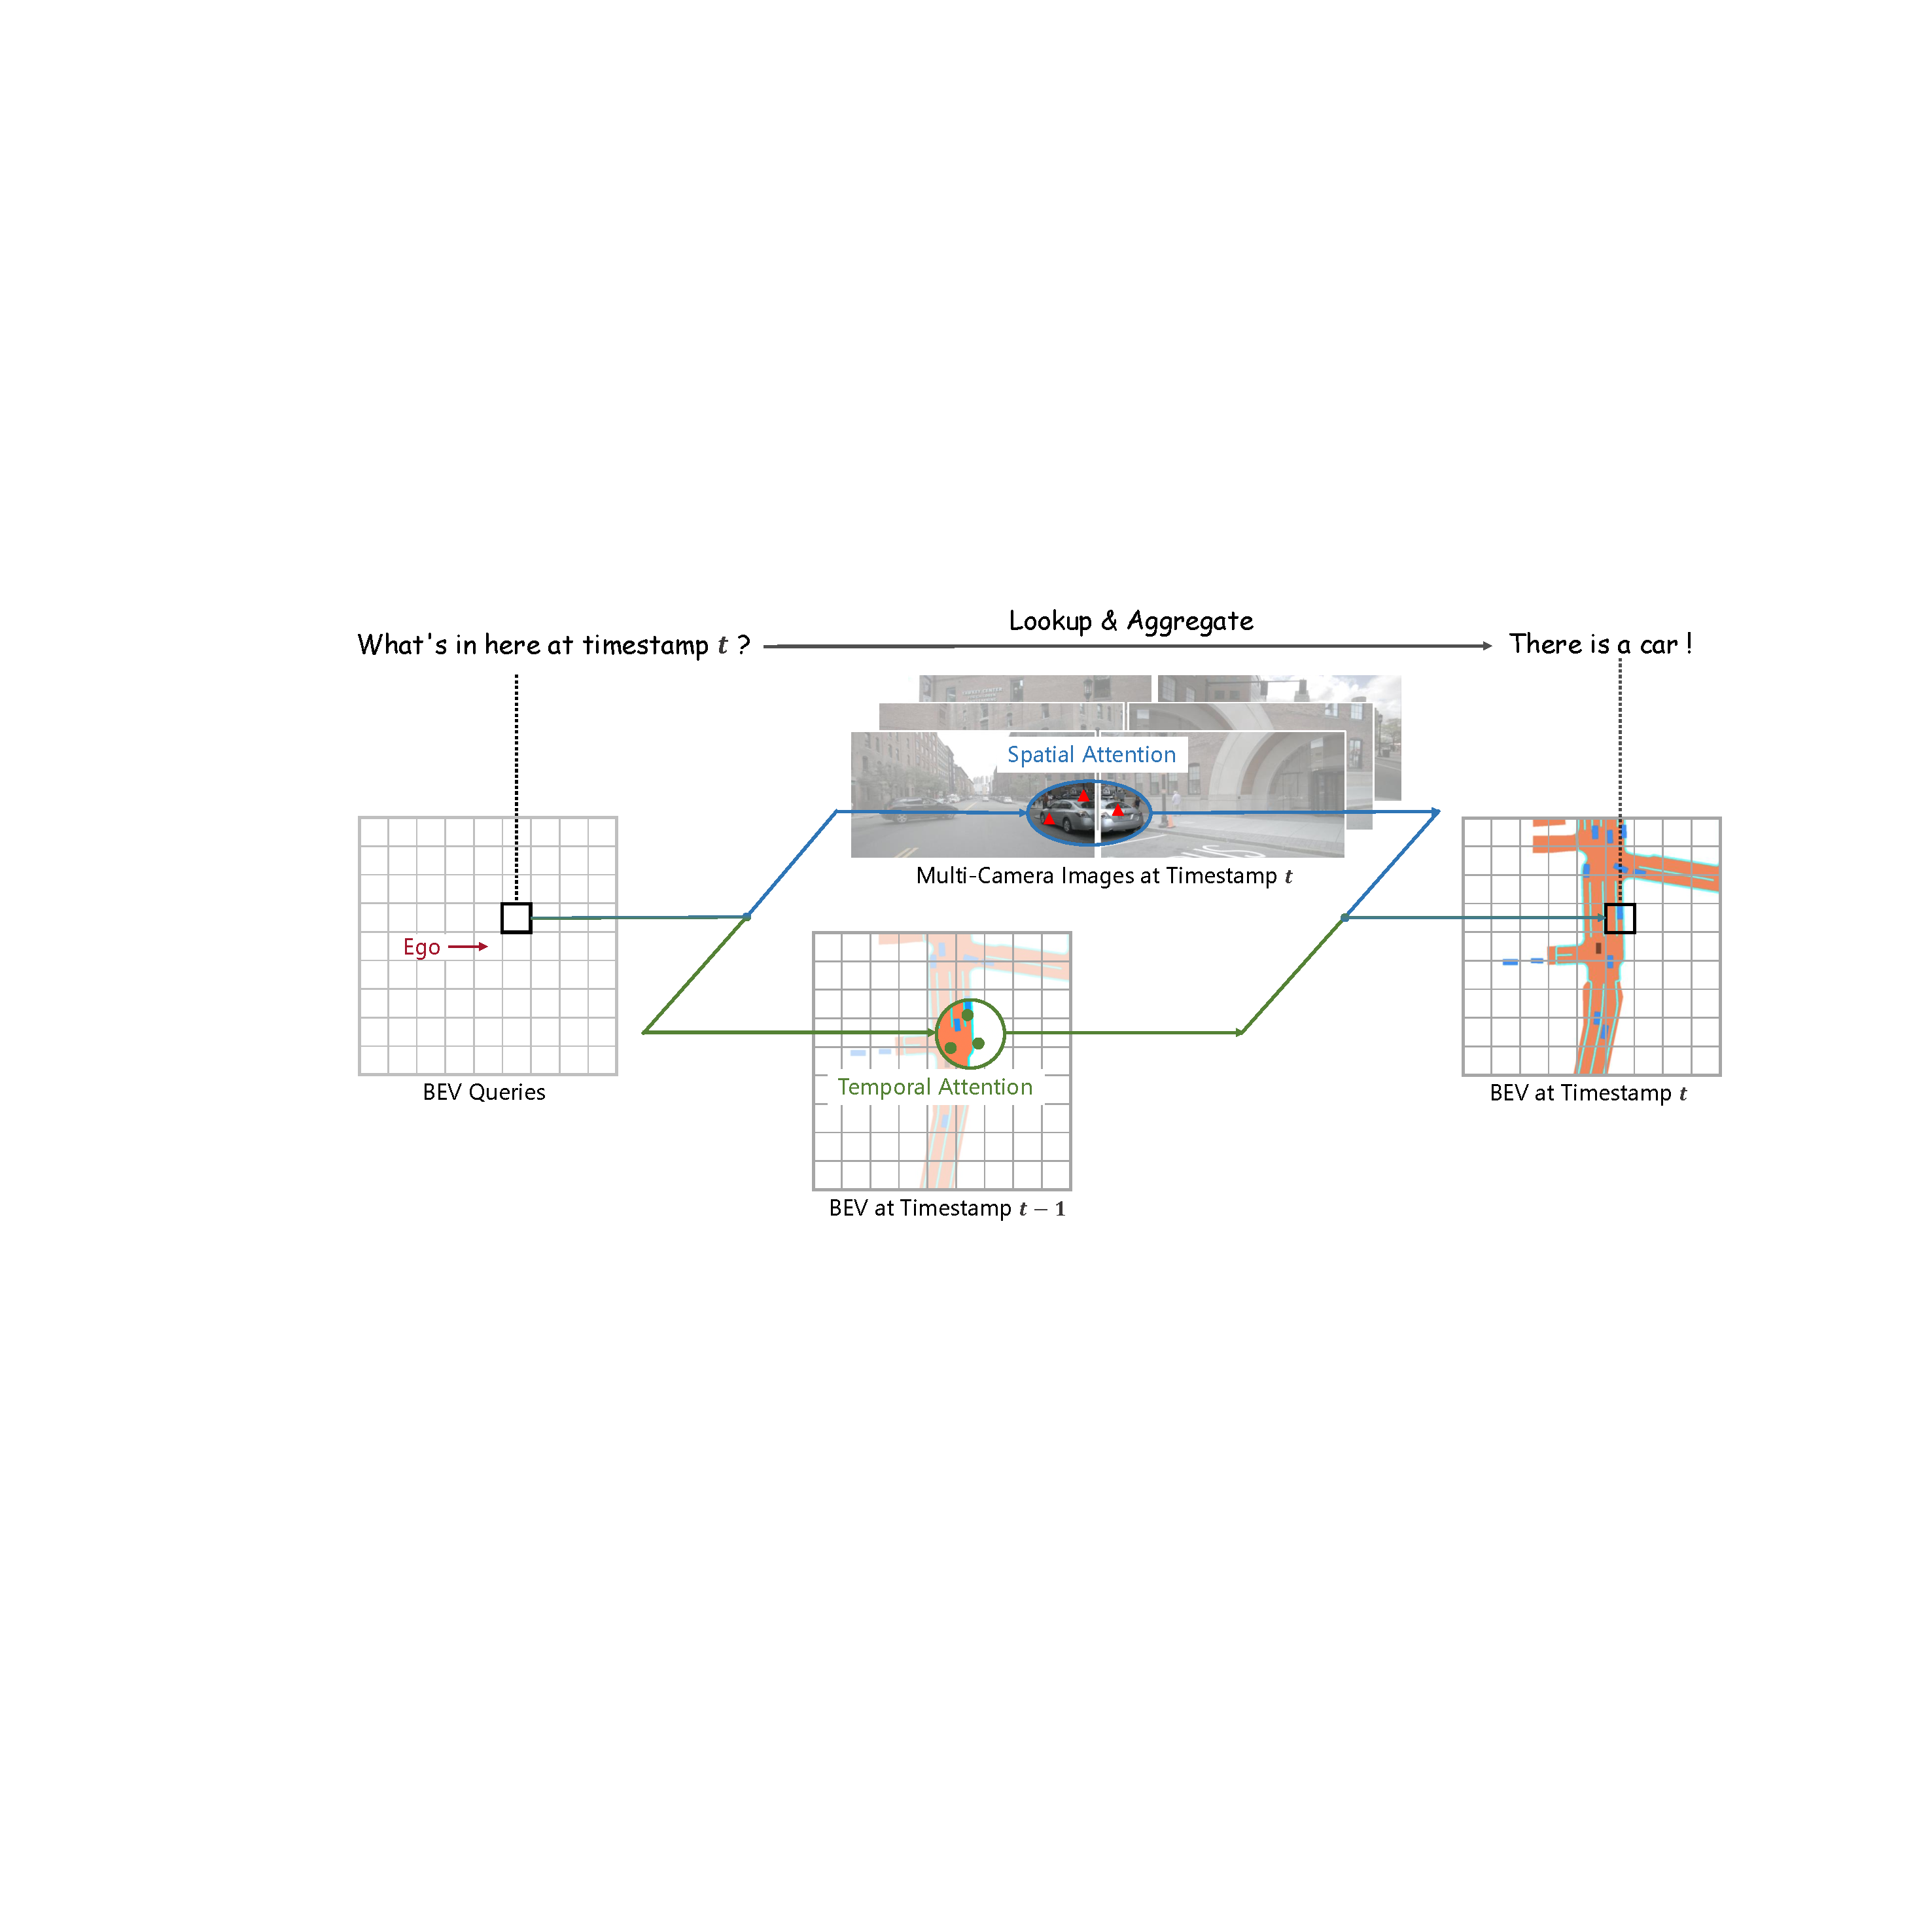
\includegraphics[width=0.9\linewidth]{img/moti.pdf}
%\vspace{-3mm}
\caption{本文提出\textbf{BEVFormer}——一种用于自动驾驶的范式，
该范式同时利用Transformer和时序结构从多相机输入生成鸟瞰视图（BEV）特征。
BEVFormer利用查询（Query）在空间/时序空间中查找并相应地聚合时空信息，
从而为感知任务提供更强的特征表示。
}
\label{fig:moti}
%%\vspace{-7mm}
%%\vspace{-11mm}
\end{figure}



\begin{abstract}
\blfootnote{*: 同等贡献（Equal contribution）。本工作完成于Zhiqi Li在上海人工智能实验室实习期间。}
\blfootnote{\Letter: 通讯作者（Corresponding author）。}
% \noindent
3D视觉感知任务（包括基于多相机图像的3D目标检测和地图分割）对于自动驾驶系统至关重要。本文提出一种名为BEVFormer的新框架，该框架通过时空Transformer学习统一的BEV表示，以支持多种自动驾驶感知任务。简而言之，BEVFormer通过预定义的网格状BEV查询与空间和时序空间交互，从而利用空间和时序信息。为聚合空间信息，本文设计了空间交叉注意力（Spatial Cross-Attention），使每个BEV查询从跨相机视图的感兴趣区域中提取空间特征。对于时序信息，本文提出了时序自注意力（Temporal Self-Attention），以循环方式融合历史BEV信息。
本文方法在nuScenes \texttt{test}集上的NDS指标达到56.9\%的当前最优（SOTA）性能，比此前最佳方法高出9.0个百分点，与基于LiDAR的基线方法性能相当。本文进一步表明，BEVFormer显著提升了速度估计精度和低可见度条件下的目标召回率。代码开源在\url{https://github.com/zhiqi-li/BEVFormer}。


\end{abstract}



\section{引言}
3D空间感知对于自动驾驶、机器人等各种应用至关重要。
%
尽管基于LiDAR的方法~\cite{vora2020pointpainting,lang2019pointpillars,zhou2018voxelnet,yan2018second,chen2017multi}取得了显著进展，
%
基于相机的方法~\cite{wang2021fcos3d,philion2020lift,wang2022detr3d,pan2020cross}近年来受到广泛关注。
与基于LiDAR的方法相比，相机除了部署成本低之外，还具有检测远距离物体和识别基于视觉的道路元素（如交通灯、停止线）的显著优势。


自动驾驶中周围场景的视觉感知需要从多相机提供的2D线索中预测3D边界框或语义地图。最直接的解决方案基于单目框架~\cite{wang2021fcos3d,wang2022probabilistic,park2021pseudo,reiher2020sim2real,bruls2019right}和跨相机后处理。该框架的缺点在于分别处理不同视角的图像，无法捕捉跨相机的信息，导致性能和效率低下~\cite{philion2020lift,wang2022detr3d}。




作为单目框架的替代方案，一种更统一的框架是从多相机图像中提取整体表示。
%
鸟瞰视图（BEV）是周围场景的常用表示形式，因为它能清晰呈现物体的位置和尺度，适用于多种自动驾驶任务（如感知和规划）~\cite{ng2020bev}。
尽管先前的地图分割方法已经证明了BEV的有效性~\cite{philion2020lift,hu2021fiery,ng2020bev}，但基于BEV的方法在3D目标检测中并未展现出相对于其他范式的显著优势~\cite{wang2022detr3d,park2021pseudo,reading2021categorical}。
根本原因在于3D目标检测任务需要强大的BEV特征来支持精确的3D边界框预测，但从2D平面生成BEV是一个不适定问题。
一种流行的基于BEV的框架利用深度信息生成BEV特征~\cite{wang2019pseudo,philion2020lift,reading2021categorical}，但该范式对深度值的精度或深度分布敏感。基于BEV的方法的检测性能因此受到复合误差的影响~\cite{wang2022detr3d}，不精确的BEV特征会严重损害最终性能。因此，\emph{本文致力于设计一种不依赖深度信息、能够自适应学习BEV特征而非严格依赖3D先验的BEV生成方法。}
Transformer利用注意力机制动态聚合有价值的特征，在概念上满足本文的需求。




使用BEV特征执行感知任务的另一个动机在于，BEV是连接时序空间和空间域的理想桥梁。
%
对于人类视觉感知系统，时序信息在推断物体运动状态和识别遮挡物体方面起着至关重要的作用，许多视觉领域的工作已经证明了利用视频数据的有效性~\cite{brazil2020kinematic,ma20223d,luo2018fast,qi2021offboard,kang2016object}。
%
然而，现有的当前最优多相机3D检测方法很少利用时序信息。
%
主要挑战在于自动驾驶对时间高度敏感且场景中物体变化迅速，因此简单地堆叠跨时间戳的BEV特征会带来额外的计算成本和干扰信息，并非理想方案。
受循环神经网络（Recurrent Neural Networks, RNN）~\cite{hochreiter1997long,cho2014properties}启发，\emph{本文利用BEV特征以循环方式将时序信息从过去传递到现在，这与RNN模型中隐藏状态的精神一致。}



为此，本文提出一种基于Transformer的鸟瞰视图编码器，称为\textbf{BEVFormer}，它能够有效聚合来自多视角相机和历史BEV特征的时空特征。
BEVFormer生成的BEV特征可同时支持多种3D感知任务（如3D目标检测和地图分割），这对自动驾驶系统非常有价值。
如图\ref{fig:moti}所示，BEVFormer包含三个关键设计：
（1）网格状BEV查询，通过注意力机制灵活融合空间和时序特征；
（2）空间交叉注意力模块，用于聚合多相机图像的空间特征；
（3）时序自注意力模块，用于从历史BEV特征中提取时序信息，有助于运动物体的速度估计和严重遮挡物体的检测，且仅带来可忽略的计算开销。
借助BEVFormer生成的统一特征，模型可与不同的任务特定头（如Deformable DETR~\cite{zhu2020deformable}和掩码解码器~\cite{li2021panoptic}）协同工作，实现端到端的3D目标检测和地图分割。 



本文主要贡献如下：

$\bullet$ 提出BEVFormer——一种时空Transformer编码器，将多相机和/或多时间戳输入投影到BEV表示中。借助统一的BEV特征，模型可同时支持多种自动驾驶感知任务，包括3D目标检测和地图分割。

$\bullet$ 设计了可学习的BEV查询，与空间交叉注意力层和时序自注意力层配合，分别从跨相机视图和历史BEV中查找空间特征和时序特征，然后聚合到统一的BEV特征中。

$\bullet$ 在多个具有挑战性的基准测试（包括nuScenes~\cite{caesar2020nuscenes}和Waymo~\cite{sun2020scalability}）上评估了BEVFormer性能。BEVFormer相比于先前方法持续取得改进。例如，在可比的参数量和计算开销下，BEVFormer在nuScenes \texttt{test}集上达到56.9\%的NDS，比此前最佳检测方法DETR3D~\cite{wang2022detr3d}高出9.0个百分点（56.9\% \emph{vs.} 47.9\%）。在地图分割任务中，本文方法同样达到当前最优性能，在最具有挑战性的车道分割任务上比Lift-Splat~\cite{philion2020lift}高出5.0个百分点以上。
希望这种简洁而强大的框架能为后续3D感知任务提供新的基线。

\section{相关工作}

\subsection{基于Transformer的2D感知}
近来，使用Transformer重构检测和分割任务已成为一种新趋势~\cite{carion2020end,zhu2020deformable,li2021panoptic}。

DETR~\cite{carion2020end}通过交叉注意力解码器直接使用一组目标查询（Object Queries）生成检测结果。
然而，DETR的主要缺点是训练时间较长。Deformable DETR~\cite{zhu2020deformable}通过提出可变形注意力（Deformable Attention）解决了这一问题。
%
与DETR中的标准全局注意力不同，可变形注意力与局部感兴趣区域交互，仅在每个参考点附近采样$K$个点并计算注意力结果，从而实现了高效率并显著缩短了训练时间。可变形注意力机制的计算公式如下：
%%\vspace{-1mm}
\begin{equation}
\text{DeformAttn}(q, p, x) = \sum_{i=1}^{N_\text{head}} \mathcal{W}_i\sum_{j=1}^{N_\text{key}} \mathcal{A}_{ij} \cdot \mathcal{W}'_i x(p+ \Delta p_{ij}),
\label{eq:single_deform_attn_fun}
%\vspace{-2mm}
\end{equation}
其中$q$、$p$、$x$分别表示查询、参考点和输入特征。$i$索引注意力头，$N_\text{head}$表示注意力头的总数。
%
$j$索引采样键，$N_\text{key}$是每个头的总采样键数量。
%
$W_i\!\in\!\mathbb{R}^{C\times (C / H_{\rm head})}$和$W'_i\!\in\!\mathbb{R}^{(C / H_{\rm head})\times C}$是可学习权重，$C$为特征维度。$A_{ij}\!\in\![0,1]$是预测的注意力权重，通过$\sum_{j=1}^{N_\text{key}} A_{ij}\!= \!1$归一化。$\Delta p_{ij}\!\in\!\mathbb{R}^2$是相对于参考点$p$的预测偏移量。$x(p + \Delta p_{ij})$表示位置$p + \Delta p_{ij}$处的特征，通过双线性插值提取（如Dai~\etal~\cite{dai2017deformable}所述）。
本文将可变形注意力扩展到3D感知任务，以高效聚合空间和时序信息。

\subsection{基于相机的3D感知}
先前的3D感知方法通常独立执行3D目标检测或地图分割任务。
在3D目标检测任务中，早期方法与2D检测方法相似~\cite{brazil2019m3d,mousavian20173d,xu2018multi,Simonelli_2019_ICCV,zhou2019objects}，通常基于2D边界框预测3D边界框。
Wang~\etal~\cite{wang2021fcos3d}借鉴先进的2D检测器FCOS~\cite{tian2019fcos}，直接预测每个物体的3D边界框。DETR3D~\cite{wang2022detr3d}将可学习的3D查询投影到2D图像上，然后采样相应特征进行端到端的3D边界框预测，无需NMS后处理。
另一种方案是将图像特征转换为BEV特征，从俯视图预测3D边界框。这类方法通过深度估计~\cite{wang2019pseudo}或类别深度分布~\cite{reading2021categorical}提供的深度信息将图像特征转换到BEV特征。
OFT~\cite{Roddick2019OrthographicFT}和ImVoxelNet~\cite{rukhovich2022imvoxelnet}将预定义体素投影到图像特征上，生成场景的体素表示。最近，M$^2$BEV~\cite{xie2022m}进一步探索了基于BEV特征同时执行多种感知任务的可行性。


事实上，从多相机特征生成BEV特征在地图分割任务中得到了更广泛的研究~\cite{philion2020lift,pan2020cross}。一种直接的方法是通过逆透视映射（Inverse Perspective Mapping, IPM）~\cite{reiher2020sim2real,can2021structured}将透视图转换为BEV。此外，Lift-Splat~\cite{philion2020lift}基于深度分布生成BEV特征。
方法~\cite{pan2020cross,hendy2020fishing,chitta2021neat}利用多层感知机学习从透视图到BEV的转换。
PYVA~\cite{yang2021projecting}提出了跨视角Transformer，将前视单目图像转换为BEV，但由于全局注意力机制~\cite{vaswani2017attention}的计算开销，该范式不适合融合多相机特征。除空间信息外，先前的工作~\cite{hu2021fiery,saha2021translating,can2020understanding}也通过堆叠多个时间戳的BEV特征来考虑时序信息。堆叠BEV特征将可用时序信息限制在固定时间窗口内，并带来额外计算开销。
本文提出的时空Transformer通过同时考虑空间和时序线索生成当前时刻的BEV特征，时序信息以RNN方式从前一时刻的BEV特征中获得，仅带来很小的计算成本。


%\vspace{-1mm}
\section{BEVFormer}
%\vspace{-1mm}
将多相机图像特征转换为鸟瞰视图（BEV）特征可以为各种自动驾驶感知任务提供统一的环境表示。
本文提出一种新的基于Transformer的BEV生成框架，通过注意力机制有效聚合多视角相机和历史BEV特征的时空信息。


\begin{figure}[t]
\centering
% 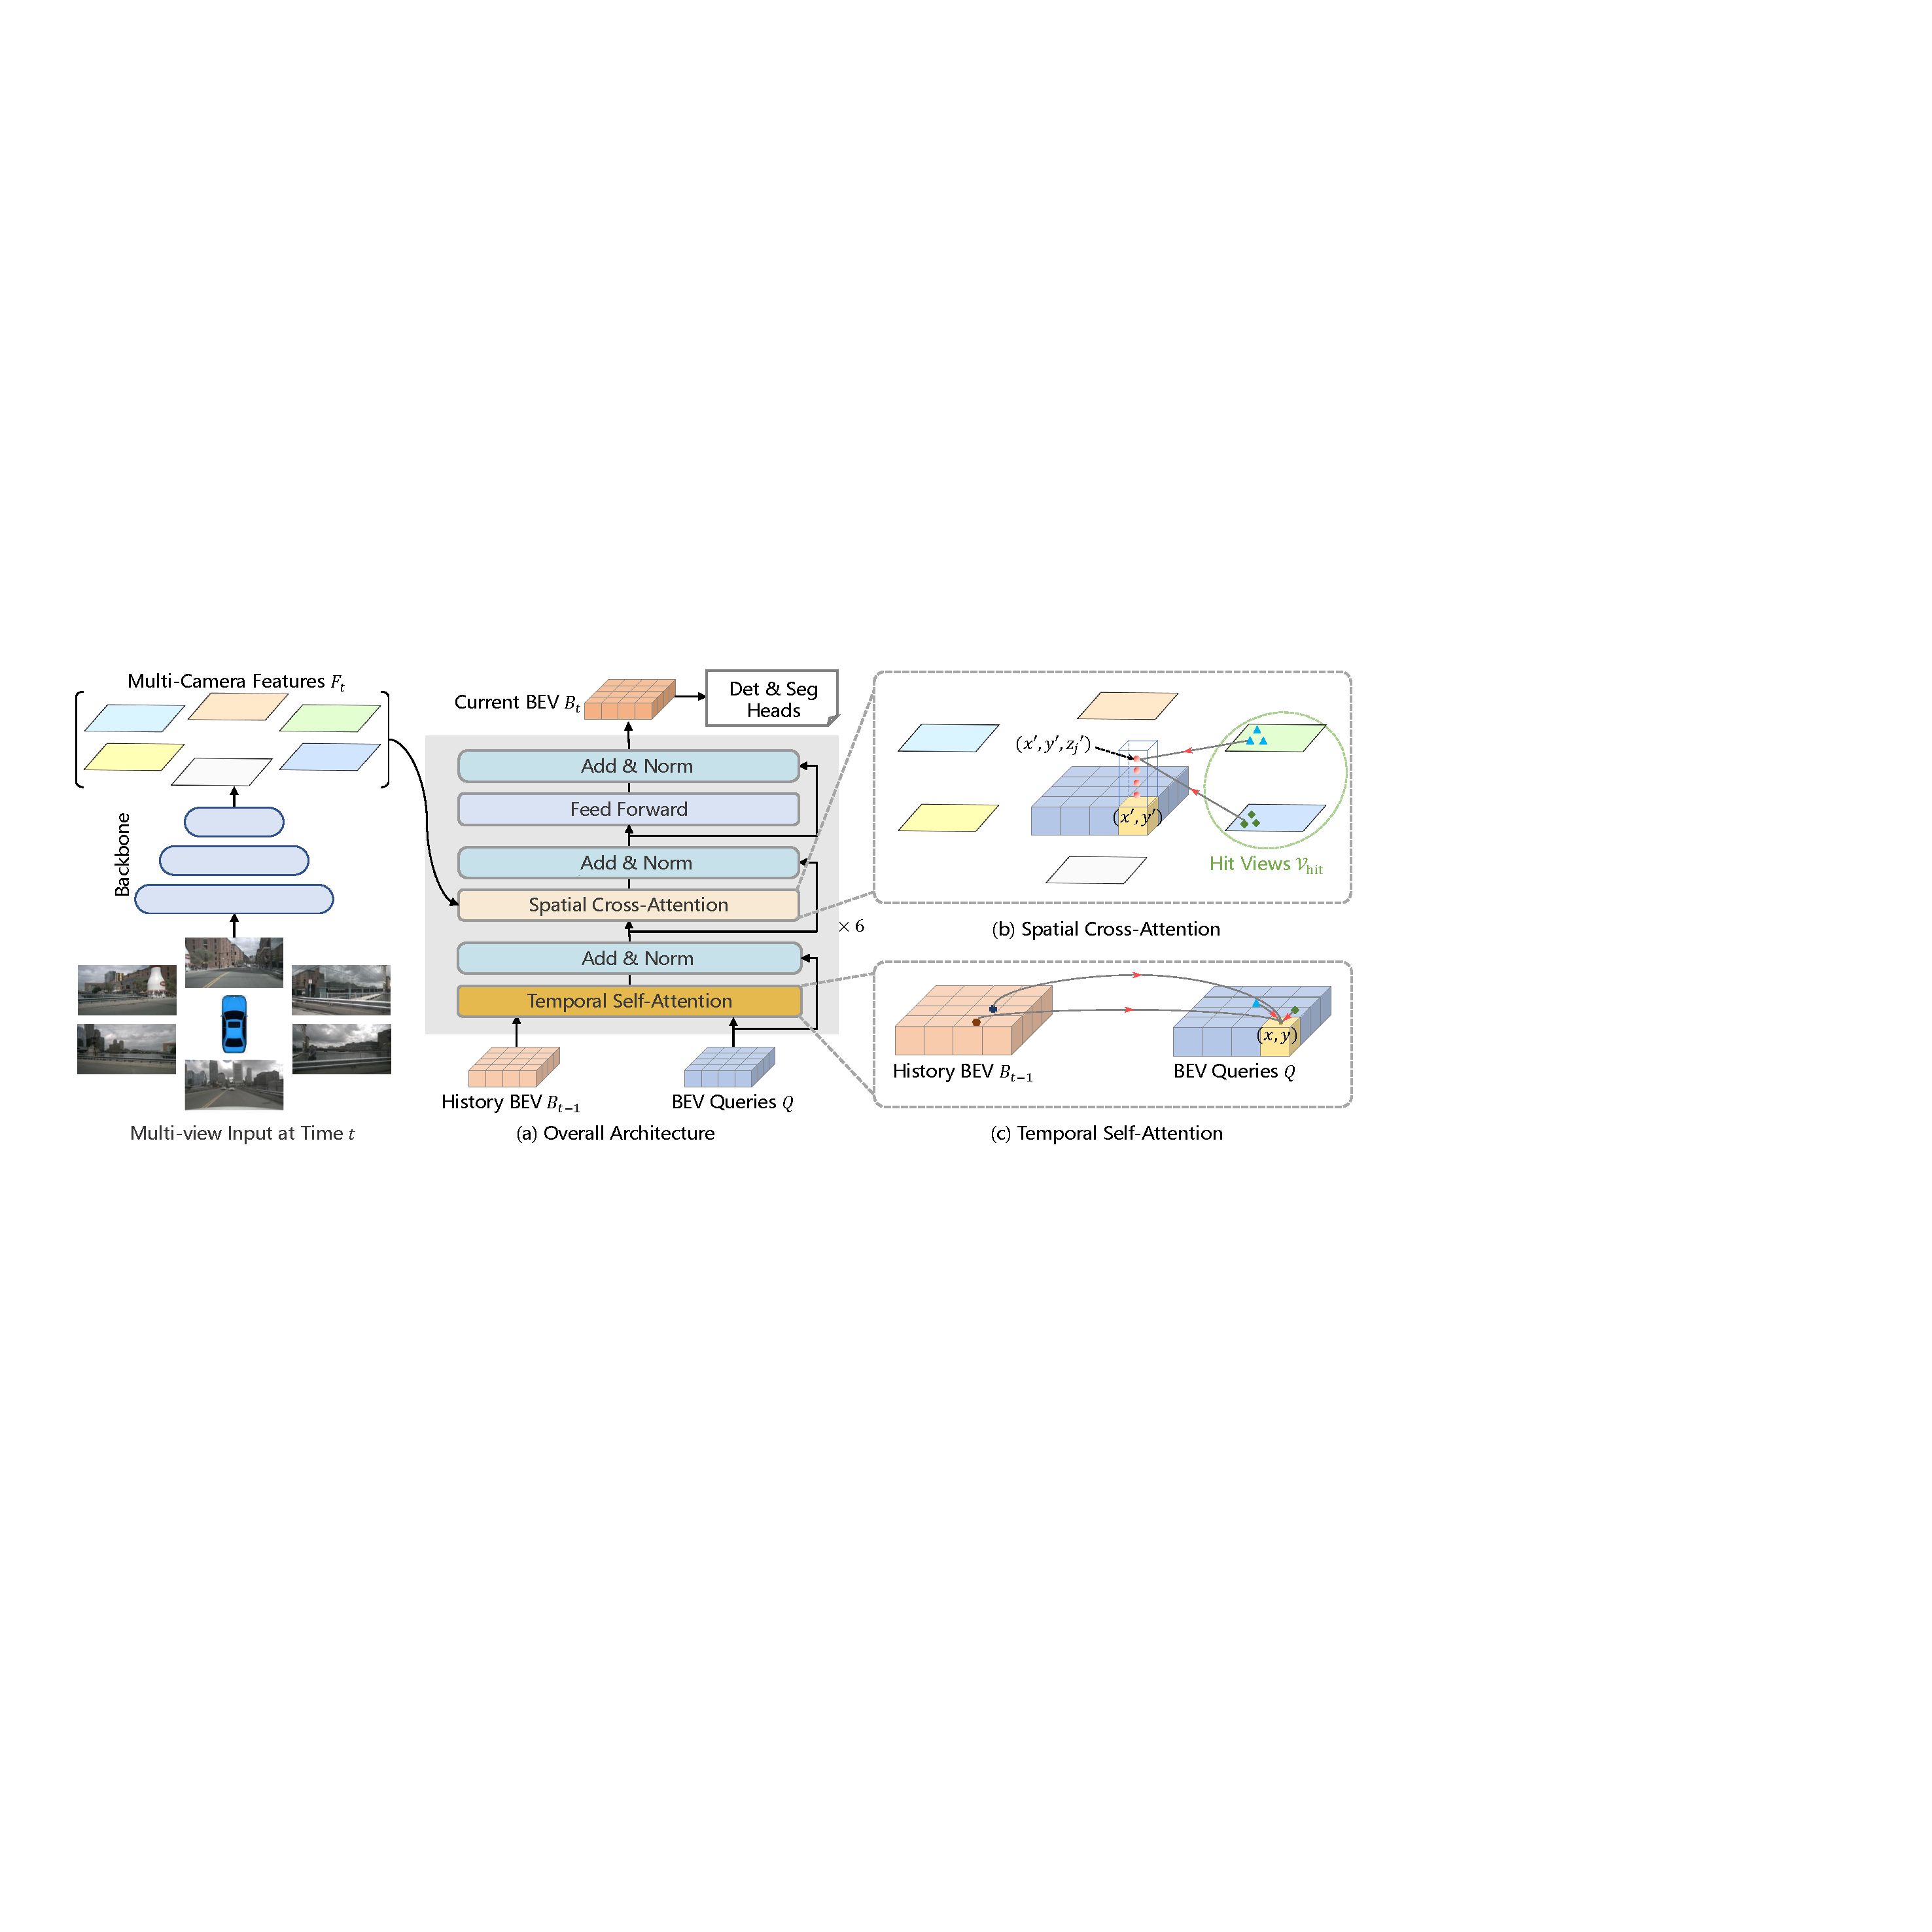
\includegraphics[width=\linewidth]{img/model.pdf}
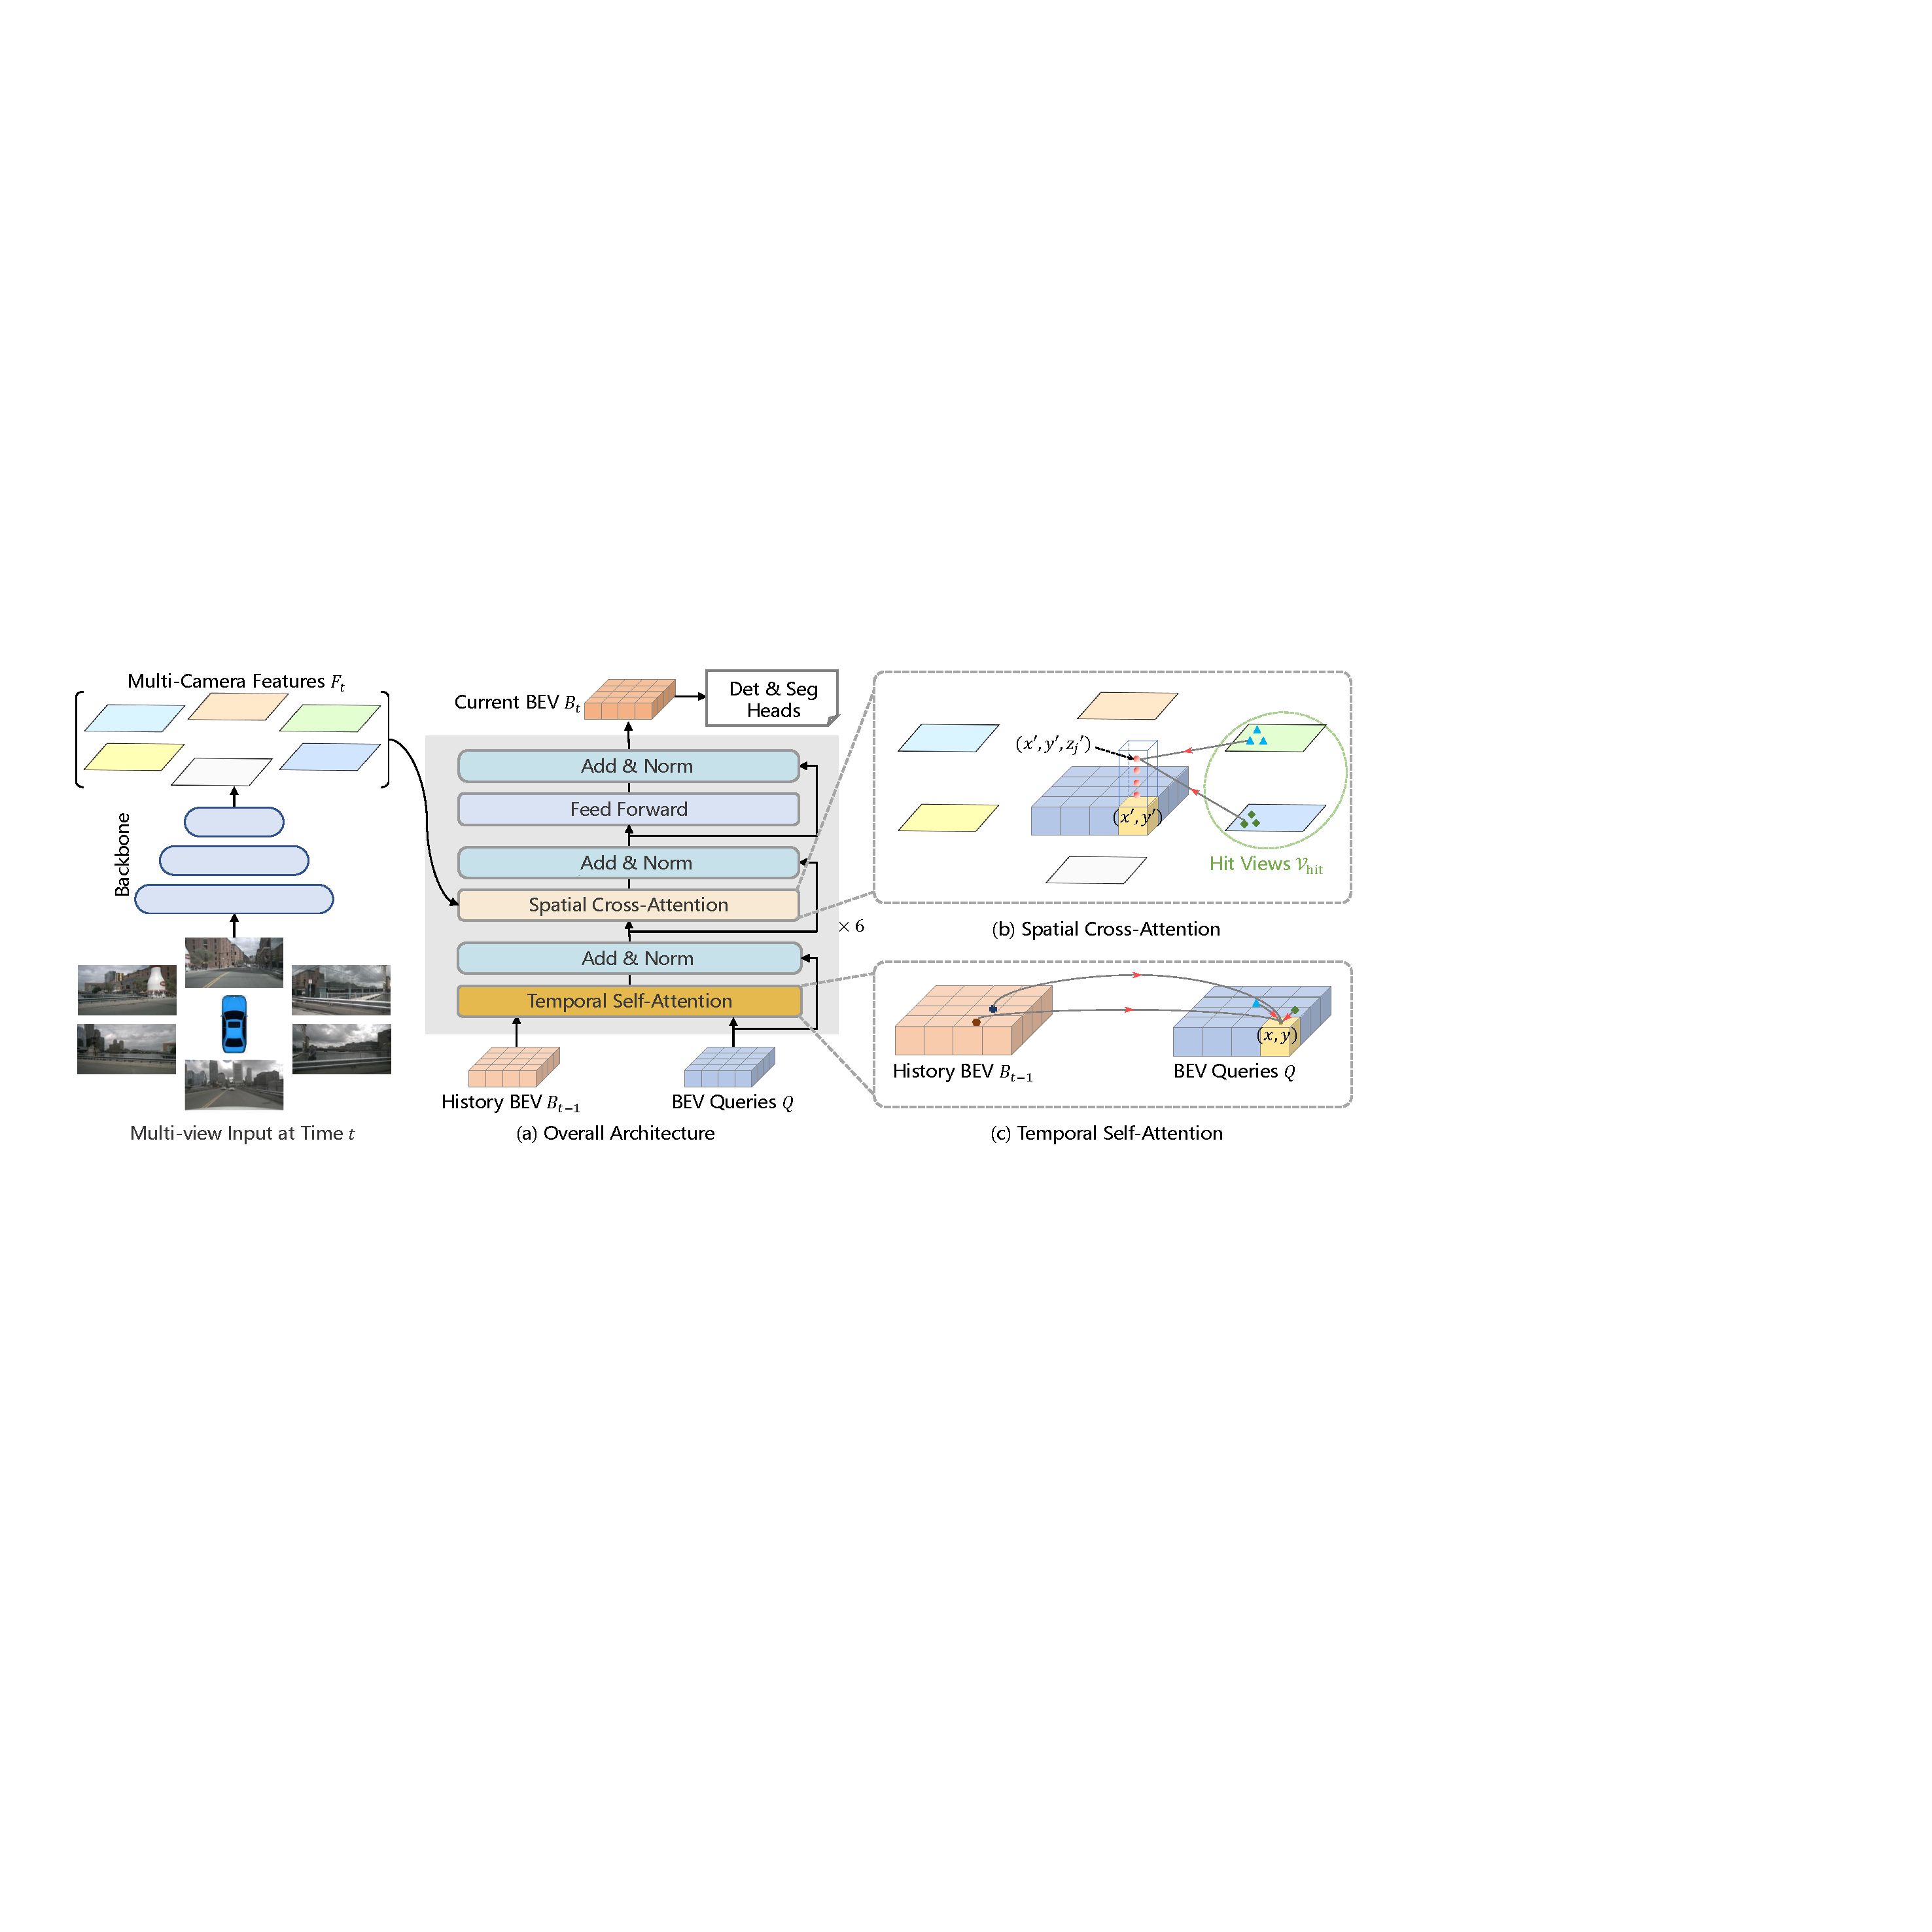
\includegraphics[width=\linewidth]{img/model.pdf}
\caption{\textbf{BEVFormer整体架构。} (a) BEVFormer的编码器层包含网格状BEV查询、时序自注意力和空间交叉注意力。 (b) 在空间交叉注意力中，每个BEV查询仅与感兴趣区域内的图像特征交互。 (c) 在时序自注意力中，每个BEV查询与两类特征交互：当前时间戳的BEV查询和前一时刻的BEV特征。}
\label{fig:model}
%\vspace{-5mm}
\end{figure}

%\vspace{-2mm}
\subsection{整体架构}
%\vspace{-1mm}
如图\ref{fig:model}所示，BEVFormer包含6个编码器层，每层遵循Transformer的传统结构~\cite{vaswani2017attention}，但包含三个特殊设计：BEV查询、空间交叉注意力和时序自注意力。
具体而言，BEV查询是网格状可学习参数，旨在通过注意力机制从多相机视角中查询BEV空间中的特征。空间交叉注意力和时序自注意力是与BEV查询配合工作的注意力层，用于根据BEV查询查找并聚合来自多相机图像的空间特征以及来自历史BEV的时序特征。



在推理过程中，在时间戳$t$处，将多相机图像输入骨干网络（如ResNet-101~\cite{he2016deep}），获得不同相机视角的特征$F_t\!=\!\{F_t^i\}_{i=1}^{N_{\rm view}}$，其中$F_t^i$是第$i$个视角的特征，$N_{\rm view}$是相机视角总数。同时，保留前一时刻$t-1$的BEV特征$B_{t\!-\!1}$。
%
%
在每个编码器层中，首先使用BEV查询$Q$通过时序自注意力从前一BEV特征$B_{t\!-\!1}$中查询时序信息。然后使用BEV查询$Q$通过空间交叉注意力从多相机特征$F_t$中查询空间信息。经过前馈网络~\cite{vaswani2017attention}后，编码器层输出精炼后的BEV特征，作为下一编码器层的输入。
经过6个堆叠的编码器层后，生成当前时间戳$t$的统一BEV特征$B_t$。以BEV特征$B_t$为输入，3D检测头和地图分割头预测3D边界框和语义图等感知结果。




%\vspace{-2mm}
\subsection{BEV查询}\label{bev_queries}
%\vspace{-1mm}
本文预定义一组网格状可学习参数$Q\!\in\! \mathbb{R}^{H\!\times\!W\!\times\!C}$作为BEVFormer的查询，其中$H,W$是BEV平面的空间形状。具体来说，位于$Q$中$p=(x,y)$处的查询$Q_p\!\in\!\mathbb{R}^{1\!\times\!C}$负责BEV平面中对应的网格单元区域。BEV平面中的每个网格单元对应实际空间中的$s$米。默认情况下，BEV特征中心对应自车位置。遵循常见做法~\cite{gehring2017convolutional}，在将BEV查询$Q$输入BEVFormer之前，加入可学习位置编码。 


\subsection{空间交叉注意力}\label{spatial_attention}
由于多相机3D感知的输入规模较大（包含$N_\text{view}$个相机视角），标准多头注意力~\cite{vaswani2017attention}的计算开销极高。
因此，本文基于可变形注意力~\cite{zhu2020deformable}开发了空间交叉注意力，这是一种资源高效的注意力层，其中每个BEV查询$Q_p$仅与跨相机视图的感兴趣区域交互。
%
然而，可变形注意力最初为2D感知设计，因此需要针对3D场景进行一些调整。


如图\ref{fig:model} (b)所示，
首先将BEV平面上的每个查询提升为柱状查询（Pillar-like Query）~\cite{lang2019pointpillars}，从柱体中采样${N_\text{ref}}$个3D参考点，然后将这些点投影到2D视图上。对于一个BEV查询，投影后的2D点只会落在部分视图上，其他视图不会被命中。将命中的视图记为$\mathcal{V}_\text{hit}$。
之后，将这些2D点视为查询$Q_p$的参考点，从命中视图$\mathcal{V}_\text{hit}$的这些参考点周围采样特征。
最后，对采样特征进行加权求和，作为空间交叉注意力的输出。
空间交叉注意力（Spatial Cross-Attention, SCA）的过程可以表示为：
\begin{align}\label{sca}
    \text{SCA}(Q_p, F_t) &= \frac{1}{|\mathcal{V}_\text{hit}|} \sum_{i\in \mathcal{V}_\text{hit}} \sum_{j=1}^{{N_\text{ref}}}
    \text{DeformAttn}(Q_p, \mathcal{P}(p,i,j), F_t^i),
\end{align}
%
其中$i$索引相机视图，$j$索引参考点，${N_\text{ref}}$是每个BEV查询的总参考点数。$F_t^i$是第$i$个相机视图的特征。对于每个BEV查询$Q_p$，使用投影函数$\mathcal{P}(p, i, j)$获取第$i$个视图图像上的第$j$个参考点。

接下来介绍如何通过投影函数$\mathcal{P}$获得视图图像上的参考点。
首先计算$Q$中位于$p=(x,y)$处的查询$Q_p$对应的真实世界位置$(x', y')$，如公式\ref{eqn:real}所示。
\begin{equation}{\label{eqn:real}}
    x'\!=\! (x\!-\!\frac{W}{2})\!\times\! s; \quad y'\! = \!(y\!-\!\frac{H}{2})\!\times\! s,
\end{equation}

其中$H,W$是BEV查询的空间形状，$s$是BEV网格的分辨率大小，$(x',y')$是以自车位置为原点的坐标。在3D空间中，位于$(x', y')$的物体会在z轴上的高度$z'$处出现。因此预定义一组锚点高度$\{z'_j\}_{j=1}^{N_\text{ref}}$，确保能捕捉到出现在不同高度的线索。
这样，对于每个查询$Q_p$，得到一个3D参考点柱体${(x', y', z'_j)}_{j=1}^{{N_\text{ref}}}$。最后，通过相机的投影矩阵将3D参考点投影到不同图像视图上，表达为：
\begin{equation}
\begin{split}
\label{project}
\mathcal{P}(p,i,j)& = (x_{ij},y_{ij})\\
\text{where}\ z_{ij}\cdot\begin{bmatrix} x_{ij} &y_{ij} & 1 \end{bmatrix}^T&= T_i \cdot \begin{bmatrix} x' &y' &z'_j & 1 \end{bmatrix}^T .
\end{split}
\end{equation}
这里，$\mathcal{P}(p,i,j)$是从第$j$个3D点$(x', y', z'_j)$投影到第$i$个视图上的2D点，$T_i\!\in\! \mathbb{R}^{3\!\times\! 4}$是第$i$个相机的已知投影矩阵。 






%\vspace{-2mm}
\subsection{时序自注意力}\label{temporal_attention}
%%\vspace{-1mm}
除空间信息外，时序信息对于视觉系统理解周围环境也至关重要~\cite{ma20223d}。
例如，在没有时序线索的情况下，从静态图像中推断运动物体的速度或检测高度遮挡的物体具有挑战性。
为解决这一问题，本文设计了时序自注意力，通过融合历史BEV特征来表示当前环境。



给定当前时间戳$t$的BEV查询$Q$和历史BEV特征$B_{t\!-\!1}$，首先根据自车运动将$B_{t\!-\!1}$与$Q$对齐，使同一网格的特征对应相同的真实世界位置。
将对齐后的历史BEV特征$B_{t\!-\!1}$记为$B'_{t\!-\!1}$。然而，从$t-1$时刻到$t$时刻，可移动物体在真实世界中以不同的偏移量移动。在不同时间的BEV特征之间构建同一物体的精确关联具有挑战性。
因此，通过时序自注意力（Temporal Self-Attention, TSA）层建模特征之间的时序连接，表达如下：
\begin{align}\label{MSDeformAttn}
    \text{TSA}(Q_p, \{Q, B'_{t-1}\}) =
    \sum_{V\in \{Q, B'_{t-1}\}} \text{DeformAttn}(Q_p, p, V),
\end{align}
其中$Q_p$表示位于$p=(x, y)$的BEV查询。此外，与标准可变形注意力不同，时序自注意力中的偏移量$\Delta p$由$Q$和$B'_{t-1}$的拼接结果预测。
特别地，对于每个序列的第一个样本，时序自注意力将退化为无时序信息的自注意力，此时将BEV特征$\{Q, B'_{t-1}\}$替换为重复的BEV查询$\{Q, Q\}$。

与~\cite{hu2021fiery,saha2021translating,can2020understanding}中简单堆叠BEV的方法相比，时序自注意力能更有效地建模长时序依赖。BEVFormer从前一时刻的BEV特征而非多个堆叠的BEV特征中提取时序信息，因此计算成本更低，受干扰信息的影响更小。




    


\subsection{BEV特征的应用}
由于BEV特征$B_t\in \mathbb{R}^{H\times W \times C}$是一种通用的2D特征图，可用于多种自动驾驶感知任务，因此3D目标检测和地图分割任务头可以基于2D感知方法~\cite{zhu2020deformable,li2021panoptic}进行少量修改即可开发。

\noindent\textbf{3D目标检测：}基于2D检测器Deformable DETR~\cite{zhu2020deformable}设计了端到端3D检测头。修改包括：使用单尺度BEV特征$B_t$作为解码器的输入，预测3D边界框和速度而非2D边界框，仅使用$L_1$损失来监督3D边界框回归。借助该检测头，模型无需NMS后处理即可端到端预测3D边界框和速度。

\noindent\textbf{地图分割：}基于2D分割方法Panoptic SegFormer~\cite{li2021panoptic}设计了地图分割头。由于基于BEV的地图分割与常规语义分割基本相同，使用~\cite{li2021panoptic}的掩码解码器和类别固定查询来针对每个语义类别，包括轿车、车辆、道路（可行驶区域）和车道。





\subsection{实现细节}
\noindent\textbf{训练阶段。}
对于时间戳$t$处的每个样本，从过去2秒的连续序列中随机采样另外3个样本，该随机采样策略可增强自车运动的多样性~\cite{zhu2017deep}。将这4个样本的时间戳记为$t\!-\!3$、$t\!-\!2$、$t\!-\!1$和$t$。
前三个时间戳的样本负责循环生成BEV特征$\{B_{t-3}, B_{t-2}, B_{t-1}\}$，该阶段不需要梯度。对于时间戳$t\!-\!3$处的第一个样本，没有前一时刻的BEV特征，时序自注意力退化为自注意力。
在时间$t$处，模型基于多相机输入和前一BEV特征$B_{t-1}$生成BEV特征$B_t$，因此$B_t$包含跨越四个样本的时序和空间线索。最后，将BEV特征$B_t$输入检测和分割头，计算相应的损失函数。



\noindent\textbf{推理阶段。}在推理阶段，按时间顺序评估视频序列的每一帧。
保存前一时刻的BEV特征并用于下一时刻，这种在线推理策略时间效率高，与实际应用场景一致。尽管利用了时序信息，推理速度仍与其他方法相当~\cite{wang2021fcos3d,wang2022detr3d}。


\section{实验}
%\vspace{-2mm}
\subsection{数据集}
%\vspace{-1mm}
本文在两个具有挑战性的公开自动驾驶数据集上进行实验，即nuScenes数据集~\cite{caesar2020nuscenes}和Waymo开放数据集~\cite{sun2020scalability}。

\noindent\textbf{nuScenes数据集}~\cite{caesar2020nuscenes}包含1000个场景，每个场景时长约20秒，关键样本以2Hz的频率进行标注。每个样本包含来自6个相机的RGB图像，水平视场角为360°。检测任务包含来自10个类别的140万个标注3D边界框。按照~\cite{philion2020lift}中的设置执行BEV分割任务。
该数据集还提供了检测任务的官方评估指标。nuScenes的平均精度（mAP）使用地面平面上的中心距离而非3D交并比（IoU）来计算，用于匹配预测结果和真实值。nuScenes指标还包含5种真阳性指标（TP Metrics），包括ATE、ASE、AOE、AVE和AAE，分别衡量平移、尺度、朝向、速度和属性误差。
nuScenes还定义了nuScenes检测分数（NDS）：
${\rm NDS}\!=\!\frac{1}{10}[5{\rm mAP}\!+\!\sum_{{\rm mTP}\in \mathbb{TP}} (1\!-\!{\rm min}(1,{\rm mTP}))]$，以捕获nuScenes检测任务的各个方面。

\noindent\textbf{Waymo开放数据集}~\cite{sun2020scalability}是一个大规模自动驾驶数据集，包含798个训练序列和202个验证序列。需要注意的是，Waymo提供的每帧五张图像仅具有约252°的水平视场角，但提供的标注标签是自车周围360°的。在训练和验证集中，移除在任何图像上不可见的边界框。由于Waymo开放数据集规模大、帧率高~\cite{reading2021categorical}，通过从训练序列中每5帧采样一次的方式使用训练集子集，且仅检测车辆类别。
在Waymo数据集上，使用0.5和0.7的3D IoU阈值计算mAP。 

\subsection{实验设置}\label{details}
%\vspace{-1mm}
参照先前方法~\cite{wang2021fcos3d,wang2022detr3d,park2021pseudo}，采用两种骨干网络：从FCOS3D~\cite{wang2021fcos3d}检查点初始化的ResNet101-DCN~\cite{he2016deep,dai2017deformable}，以及从DD3D~\cite{park2021pseudo}检查点初始化的VoVnet-99~\cite{lee2019energy}。默认使用FPN~\cite{Lin2017FeaturePN}输出的多尺度特征，尺寸为\nicefrac{1}{16}、\nicefrac{1}{32}、\nicefrac{1}{64}，特征维度$C\!=\!256$。在nuScenes实验上，BEV查询的默认大小为$200\!\times\!200$，感知范围为$X$和$Y$轴的[$-$51.2m, 51.2m]，BEV网格的分辨率$s$为0.512m。对BEV查询采用可学习位置编码。
BEV编码器包含6个编码器层，每层不断精炼BEV查询。每个编码器层输入的BEV特征$B_{t\!-\!1}$相同且不需要梯度。对于每个局部查询，在由可变形注意力机制实现的空间交叉注意力模块中，对应${N_\text{ref}}\!=\!4$个不同高度的3D目标点，预定义的高度锚点从$-5$米到3米均匀采样。对于2D视图特征上的每个参考点，每个头在该参考点周围使用4个采样点。
默认情况下，模型训练24个轮次，学习率为$2\!\times\!10^{-4}$。

在Waymo实验上更改了一些设置。由于Waymo的相机系统无法捕获自车周围的完整场景~\cite{sun2020scalability}，BEV查询的默认空间形状为$300\!\times\!220$，$X$轴感知范围为[$-$35.0m, 75.0m]，$Y$轴感知范围为[$-$75.0m, 75.0m]。每个网格的分辨率$s$为0.5m。自车位于BEV的(70, 150)处。

\noindent\textbf{基线方法。}为消除任务头的影响并公平比较其他BEV生成方法，使用VPN~\cite{pan2020cross}和Lift-Splat~\cite{philion2020lift}替换BEVFormer，保持任务头和其他设置不变。还将BEVFormer调整为静态模型\textbf{BEVFormer-S}，将时序自注意力改为不使用历史BEV特征的标准自注意力。


\begin{table}[t]
\begin{center}
\caption{
\textbf{nuScenes \texttt{test}集上的3D检测结果。} $*$表示VoVNet-99 (V2-99)~\cite{lee2019energy}在深度估计任务上使用额外数据~\cite{park2021pseudo}进行了预训练。``BEVFormer-S''表示在BEV编码器中不利用时序信息。``L''和``C''分别表示LiDAR和Camera。
}

\setlength{\tabcolsep}{0.28mm}
\begin{tabular}{l  c c |c c| c c c c c c }
\toprule
方法 &  模态 & 骨干网络 & NDS$\uparrow$  & mAP$\uparrow$  & mATE$\downarrow$     & mASE$\downarrow$     & mAOE$\downarrow$     & mAVE$\downarrow$    & mAAE$\downarrow$    \\
\midrule

%\rowcolor{gray95}
SSN~\cite{zhu2020ssn} &L &-& 0.569 &0.463 &-&-&-&-&-\\
%\rowcolor{gray95}
CenterPoint-Voxel~\cite{yin2021center} & L &-& 0.655 & 0.580  & - &- &- &- &- \\
PointPainting~\cite{vora2020pointpainting}& L$\!\&\!$C&-&0.581 &0.464 &0.388&0.271&0.496&0.247&0.111\\
\midrule

FCOS3D~\cite{wang2021fcos3d}  & C  & R101& 0.428 &0.358& 0.690& 0.249& 0.452& 1.434 &\textbf{0.124} \\
PGD~\cite{wang2022probabilistic}  & C &  R101&0.448 &0.386& \textbf{0.626}& \textbf{0.245} &0.451 &1.509 &0.127 \\
%M$^2$BEV  & C & X101~\cite{xie2017aggregated}& 0.451& 0.398 &0.577 &\textbf{0.245}&0.500&1.227&0.154\\
%\midrule
\rowcolor{gray95}
BEVFormer-S    & C & R101& 0.462& 0.409 & 0.650 & 0.261 & 0.439 & 0.925 & 0.147 \\
\rowcolor{gray9}
BEVFormer    & C & R101& \textbf{0.535}& \textbf{0.445} & 0.631 & 0.257 & \textbf{0.405} & \textbf{0.435} & 0.143 \\
\midrule
DD3D~\cite{park2021pseudo}  & C &V2-99$^*$& 0.477 &0.418& \textbf{0.572} & \textbf{0.249} &\textbf{0.368} &1.014 &\textbf{0.124} \\

DETR3D~\cite{wang2022detr3d}  & C &  V2-99$^*$& 0.479 & 0.412 &0.641& 0.255 &0.394 &0.845& 0.133\\
%BEVDet  & Camera & $\ddag$V2-99& 0.488 &0.424 &\textbf{0.524} &\textbf{0.242} &0.373 &0.950&0.148\\
\rowcolor{gray95}
BEVFormer-S& C &V2-99$^*$ & 0.495& 0.435 & 0.589&0.254 & 0.402 &0.842 & 0.131 \\
\rowcolor{gray9}
BEVFormer& C &V2-99$^*$ & \textbf{0.569}& \textbf{0.481} & 0.582&0.256 & 0.375 & \textbf{0.378} & 0.126 \\

\bottomrule
\end{tabular}
% }
\label{main_det}
\end{center}
%\vspace{-4mm}
\end{table}
\begin{table}[t]
\begin{center}
\caption{
\textbf{nuScenes \texttt{val}集上的3D检测结果。} ``C''表示Camera。
}

\setlength{\tabcolsep}{0.87mm}
\begin{tabular}{l  c c |c c| c c c c c c  }
\toprule
方法 &  模态 & 骨干网络 & NDS$\uparrow$  & mAP$\uparrow$  & mATE$\downarrow$     & mASE$\downarrow$     & mAOE$\downarrow$     & mAVE$\downarrow$    & mAAE$\downarrow$    \\
\midrule


%BEVDet & val & Camera& R101 & 0.389 &0.317 &0.704 &0.273 &0.531 &0.940 &0.250\\
FCOS3D~\cite{wang2021fcos3d}&  C & R101& 0.415 & 0.343 & 0.725 & 0.263 & 0.422 & 1.292  &\textbf{0.153}  \\
PGD~\cite{wang2022probabilistic} & C &R101 & 0.428 &0.369 &0.683 &\textbf{0.260}& 0.439 &1.268 &0.185 \\
DETR3D~\cite{wang2022detr3d}& C& R101 & 0.425 &0.346 &0.773 &0.268 &0.383 &0.842 &0.216\\
%DETR3D & Camera & 0.434& 0.349 &0.716& 0.268 &0.379 &0.842& 0.200\\

%\midrule

%Lift-Splat* & val & Camera & R101 & 0.397 & 0.348 & 0.784 & 0.284 & 0.537 & 0.938 & 0.229 \\
%VPN* & val & Camear & R101 & 0.356 & 0.278 & 0.911 & 0.288 & 0.519 &0.886 & 0.227\\
\rowcolor{gray95}
BEVFormer-S & C & R101& 0.448 & 0.375 & 0.725 & 0.272 & 0.391 & 0.802 & 0.200\\
%BEVFormer (Ours)& val  & Camera & R101& 0.490& 0.378 & 0.728 & 0.280 & 0.385 & 0.400 & 0.199\\
\rowcolor{gray9}
BEVFormer   & C & R101& \textbf{0.517}& \textbf{0.416} & \textbf{0.673} & 0.274 & \textbf{0.372} & \textbf{0.394} & 0.198 \\
\bottomrule
\end{tabular}
% }
\label{val_det}
\end{center}
%\vspace{-9mm}
\end{table}

\begin{table}[t] 
\begin{center}
\caption{\textbf{在Waymo \texttt{val}集上分别使用Waymo评估指标和nuScenes评估指标的3D检测结果。} ``L1’’和``L2’’指Waymo的``LEVEL\_1’’和``LEVEL\_2’’难度~\cite{sun2020scalability}。$*$：仅使用前置相机，且仅考虑前置相机视场角（50.4°）内的物体标签。
${\text{\textdagger}}$：将ATE和AAE设为1来计算NDS分数。``L’’和``C’’分别表示LiDAR和Camera。
}

\setlength{\tabcolsep}{0.5mm}
%\resizebox{\linewidth}{!}{
\input{table/Waymo}
%}
\label{table:Waymo}
\end{center}
%\vspace{-5mm}
\end{table}



\begin{table}[t] 
\begin{center}

\caption{
\textbf{nuScenes \texttt{val}集上的3D检测和地图分割结果。}
联合训练与单独训练分割和检测任务的对比。
$*$：使用VPN~\cite{pan2020cross}和Lift-Splat~\cite{philion2020lift}替换BEV编码器进行对比，任务头相同。${\text{\textdagger}}$：来自原论文的结果。
}

\setlength{\tabcolsep}{2.9mm}
%\resizebox{\linewidth}{!}{
\begin{tabular}{l| c c | c c | c c c c }
\toprule
% \multirow{2}{*}{Clean} &\multirow{2}{*}{Mean} &
\multirow{2}{*}{方法}& \multicolumn{2}{c|}{任务头}
 & \multicolumn{2}{c|}{3D检测} & \multicolumn{4}{c}{BEV分割 (IoU)} \\
&检测& 分割& NDS$\uparrow$ &mAP$\uparrow$  & 轿车 & 各类车辆 & 道路 & 车道\\
%\multirow{2}{*}{Det} & \multirow{2}{*}{Seg} 
%Method & Modality & NDS& mAP &  IOU$_{\rm Car}$ 
\midrule
Lift-Splat$^{\text{\textdagger}}$~\cite{philion2020lift} &\xmark &\cmark &- &-& 32.1 & 32.1 & 72.9 &20.0\\
FIERY$^{\text{\textdagger}}$~\cite{hu2021fiery}&\xmark &  \cmark& - &-&- & 38.2 & - & -\\
\midrule
VPN$^*$~\cite{pan2020cross} & \cmark & \xmark & 0.333 & 0.253   &- & - &- &-\\
VPN$^*$ &\xmark &\cmark & - & -  & 31.0 & 31.8 &76.9 &19.4 \\
VPN$^*$ &\cmark & \cmark& 0.334 & 0.257  &36.6 & 37.3 & 76.0 & 18.0\\
Lift-Splat$^*$& \cmark &\xmark & 0.397 & 0.348  & -&-&-&-\\
Lift-Splat$^*$ &\xmark &\cmark &- &- &42.1 & 41.7 &77.7 & 20.0 \\
Lift-Splat$^*$& \cmark & \cmark&  0.410 & 0.344&  43.0 & 42.8 & 73.9 & 18.3\\
\rowcolor{gray95}
BEVFormer-S&\cmark & \xmark & 0.448 & 0.375&  -& - & - & -\\
\rowcolor{gray95}
BEVFormer-S& \xmark& \cmark  &- &-&43.1  &43.2  &\textbf{80.7} &21.3 \\
\rowcolor{gray95}
BEVFormer-S&\cmark & \cmark & 0.453 & 0.380 &  44.3& 44.4 & 77.6 & 19.8\\

\rowcolor{gray9}
BEVFormer&  \cmark  &\xmark & 0.517 & \textbf{0.416} &- & - & - & -\\
\rowcolor{gray9}
BEVFormer&\xmark & \cmark& - &-&44.8 & 44.8 & 80.1 & \textbf{25.7}\\
\rowcolor{gray9}
BEVFormer&\cmark & \cmark & \textbf{0.520} & 0.412 & \textbf{46.8} & \textbf{46.7} & 77.5 & 23.9\\

\bottomrule


\end{tabular}
%}
\label{table:multi-tasks}
\end{center}
%\vspace{-8mm}
\end{table}


\subsection{3D目标检测结果}

仅在检测任务上使用检测头训练模型，以便与先前的当前最优3D目标检测方法进行公平比较。
在表\ref{main_det}和表\ref{val_det}中报告了在nuScenes \texttt{test}和\texttt{val}划分上的主要结果。在公平的训练策略和可比的模型规模下，本文方法在\texttt{val}集上以9.2个百分点的优势超越此前最佳方法DETR3D~\cite{wang2022detr3d}（51.7\% NDS \emph{vs.~}42.5\% NDS）。在\texttt{test}集上，模型在无复杂技巧的情况下达到56.9\%的NDS，比DETR3D（47.9\% NDS）高出9.0个百分点。本文方法甚至可以与一些基于LiDAR的基线方法（如SSN（56.9\% NDS）~\cite{zhu2020ssn}和PointPainting（58.1\% NDS）~\cite{vora2020pointpainting}）性能相当。

此前基于相机的方法~\cite{wang2022detr3d,park2021pseudo,wang2021fcos3d}几乎无法估计速度，本文方法证明了时序信息在多相机检测的速度估计中起着至关重要的作用。
BEVFormer在\texttt{test}集上的平均速度误差（mAVE）为0.378 m/s，大幅超越其他基于相机的方法，接近基于LiDAR的方法~\cite{vora2020pointpainting}的性能。

还在Waymo上进行了实验，如表\ref{table:Waymo}所示。参照~\cite{reading2021categorical}，使用0.7和0.5的IoU阈值评估车辆类别。此外，还采用nuScenes指标评估结果，因为基于IoU的指标对基于相机的方法过于苛刻。由于只有少数基于相机的工作报告了Waymo上的结果，因此使用DETR3D的官方代码在Waymo上进行实验以便对比。可以观察到，在IoU阈值为0.5的条件下，BEVFormer在LEVEL\_1和LEVEL\_2难度上分别以6.0\%和2.5\%的带航向信息平均精度（APH）~\cite{sun2020scalability}超越DETR3D。在nuScenes指标上，BEVFormer以3.2\% NDS和5.2\% AP的优势超越DETR3D。还在前置相机上进行了实验，将BEVFormer与CaDNN~\cite{reading2021categorical}（一种在Waymo数据集上报告了结果的单目3D检测方法）进行比较。在IoU阈值为0.5的条件下，BEVFormer在LEVEL\_1和LEVEL\_2难度上分别以13.3\%和11.2\%的APH超越CaDNN。 








\subsection{多任务感知结果}
同时使用检测和分割头训练模型，以验证模型对多任务的学习能力，结果如表\ref{table:multi-tasks}所示。
在相同设置下比较不同BEV编码器时，BEVFormer在所有任务上取得了更高性能，仅道路分割结果与BEVFormer-S相当。例如，在联合训练下，BEVFormer在检测任务上以11.0个百分点的优势超越Lift-Splat$^*$~\cite{philion2020lift}（52.0\% NDS \emph{v.s.} 41.0\% NDS），在车道分割上的IoU高出5.6个百分点（23.9\% \emph{v.s.} 18.3\%）。
与单独训练任务相比，多任务学习通过共享更多模块（包括骨干网络和BEV编码器）节省了计算成本并减少了推理时间。本文表明，BEV编码器生成的BEV特征能够很好地适应不同任务，使用多任务头训练的模型在检测任务和车辆分割上表现更优。然而，联合训练模型在道路和车道分割上不如单独训练模型，这是多任务学习中一种常见的现象，称为\textit{负迁移}~\cite{crawshaw2020multi,fifty2021efficiently}。



\begin{table}[t] 
\begin{center}
\caption{\textbf{不同方法在nuScenes \texttt{val}集上使用不同BEV编码器的检测结果。} ``Memory''表示训练期间消耗的GPU显存。
$*$：使用VPN~\cite{pan2020cross}和Lift-Splat~\cite{philion2020lift}替换BEV编码器进行对比。${\text{\textdagger}}$：在空间交叉注意力中使用全局注意力训练BEVFormer-S，模型使用fp16权重训练。此外，仅采用骨干网络的单尺度特征，并将BEV查询的空间形状设为$100\!\times\!100$以节省显存。
$\ddag$：通过移除预测的偏移量和权重，将可变形注意力的交互目标从局部区域退化为仅参考点。
}

\setlength{\tabcolsep}{1.4mm}
%\resizebox{\linewidth}{!}{
\begin{tabular}{l  c |c c c c |c c c  c }
\toprule
方法 &  注意力机制 & NDS$\uparrow$  & mAP$\uparrow$  & mATE$\downarrow$    & mAOE$\downarrow$       & 参数量 &FLOPs& 显存 \\
\midrule


VPN$^*$~\cite{pan2020cross}&- & 0.334 &0.252 &0.926 &0.598 & 111.2M &924.5G &$\sim\!$20G\\
List-Splat$^*$~\cite{philion2020lift}&- &  0.397 & 0.348 &0.784 &0.537 &74.0M & 1087.7G&$\sim\!$20G \\

\midrule
\rowcolor{gray95}
BEVFormer-S$^{\text{\textdagger}}$ &Global & 0.404 & 0.325 & 0.837 &0.442&62.1M & 1245.1G& $\sim\!$36G\\ % (100*100 BEV single sacle feature C5)
\rowcolor{gray9}
BEVFormer-S$^\ddag$& Points &0.423 &0.351 &0.753&0.442  & 68.1M & 1264.3G&$\sim\!$20G\\
\rowcolor{gray85}
BEVFormer-S& Local &\textbf{0.448} &\textbf{0.375}&\textbf{0.725} &\textbf{0.391} & 68.7M &1303.5G &$\sim\!$20G\\
%\midrule
%\rowcolor{gray8}
%BEVFormer & Local & 0.517 &  0.416 &0.673 &0.372& 68.7M & 1303.5G &&$\sim\!$25G\\
\bottomrule
\end{tabular}
%}
\label{bevformer_s_abl}
\end{center}
%\vspace{-9mm}

\end{table}

\begin{figure}[t]
\centering
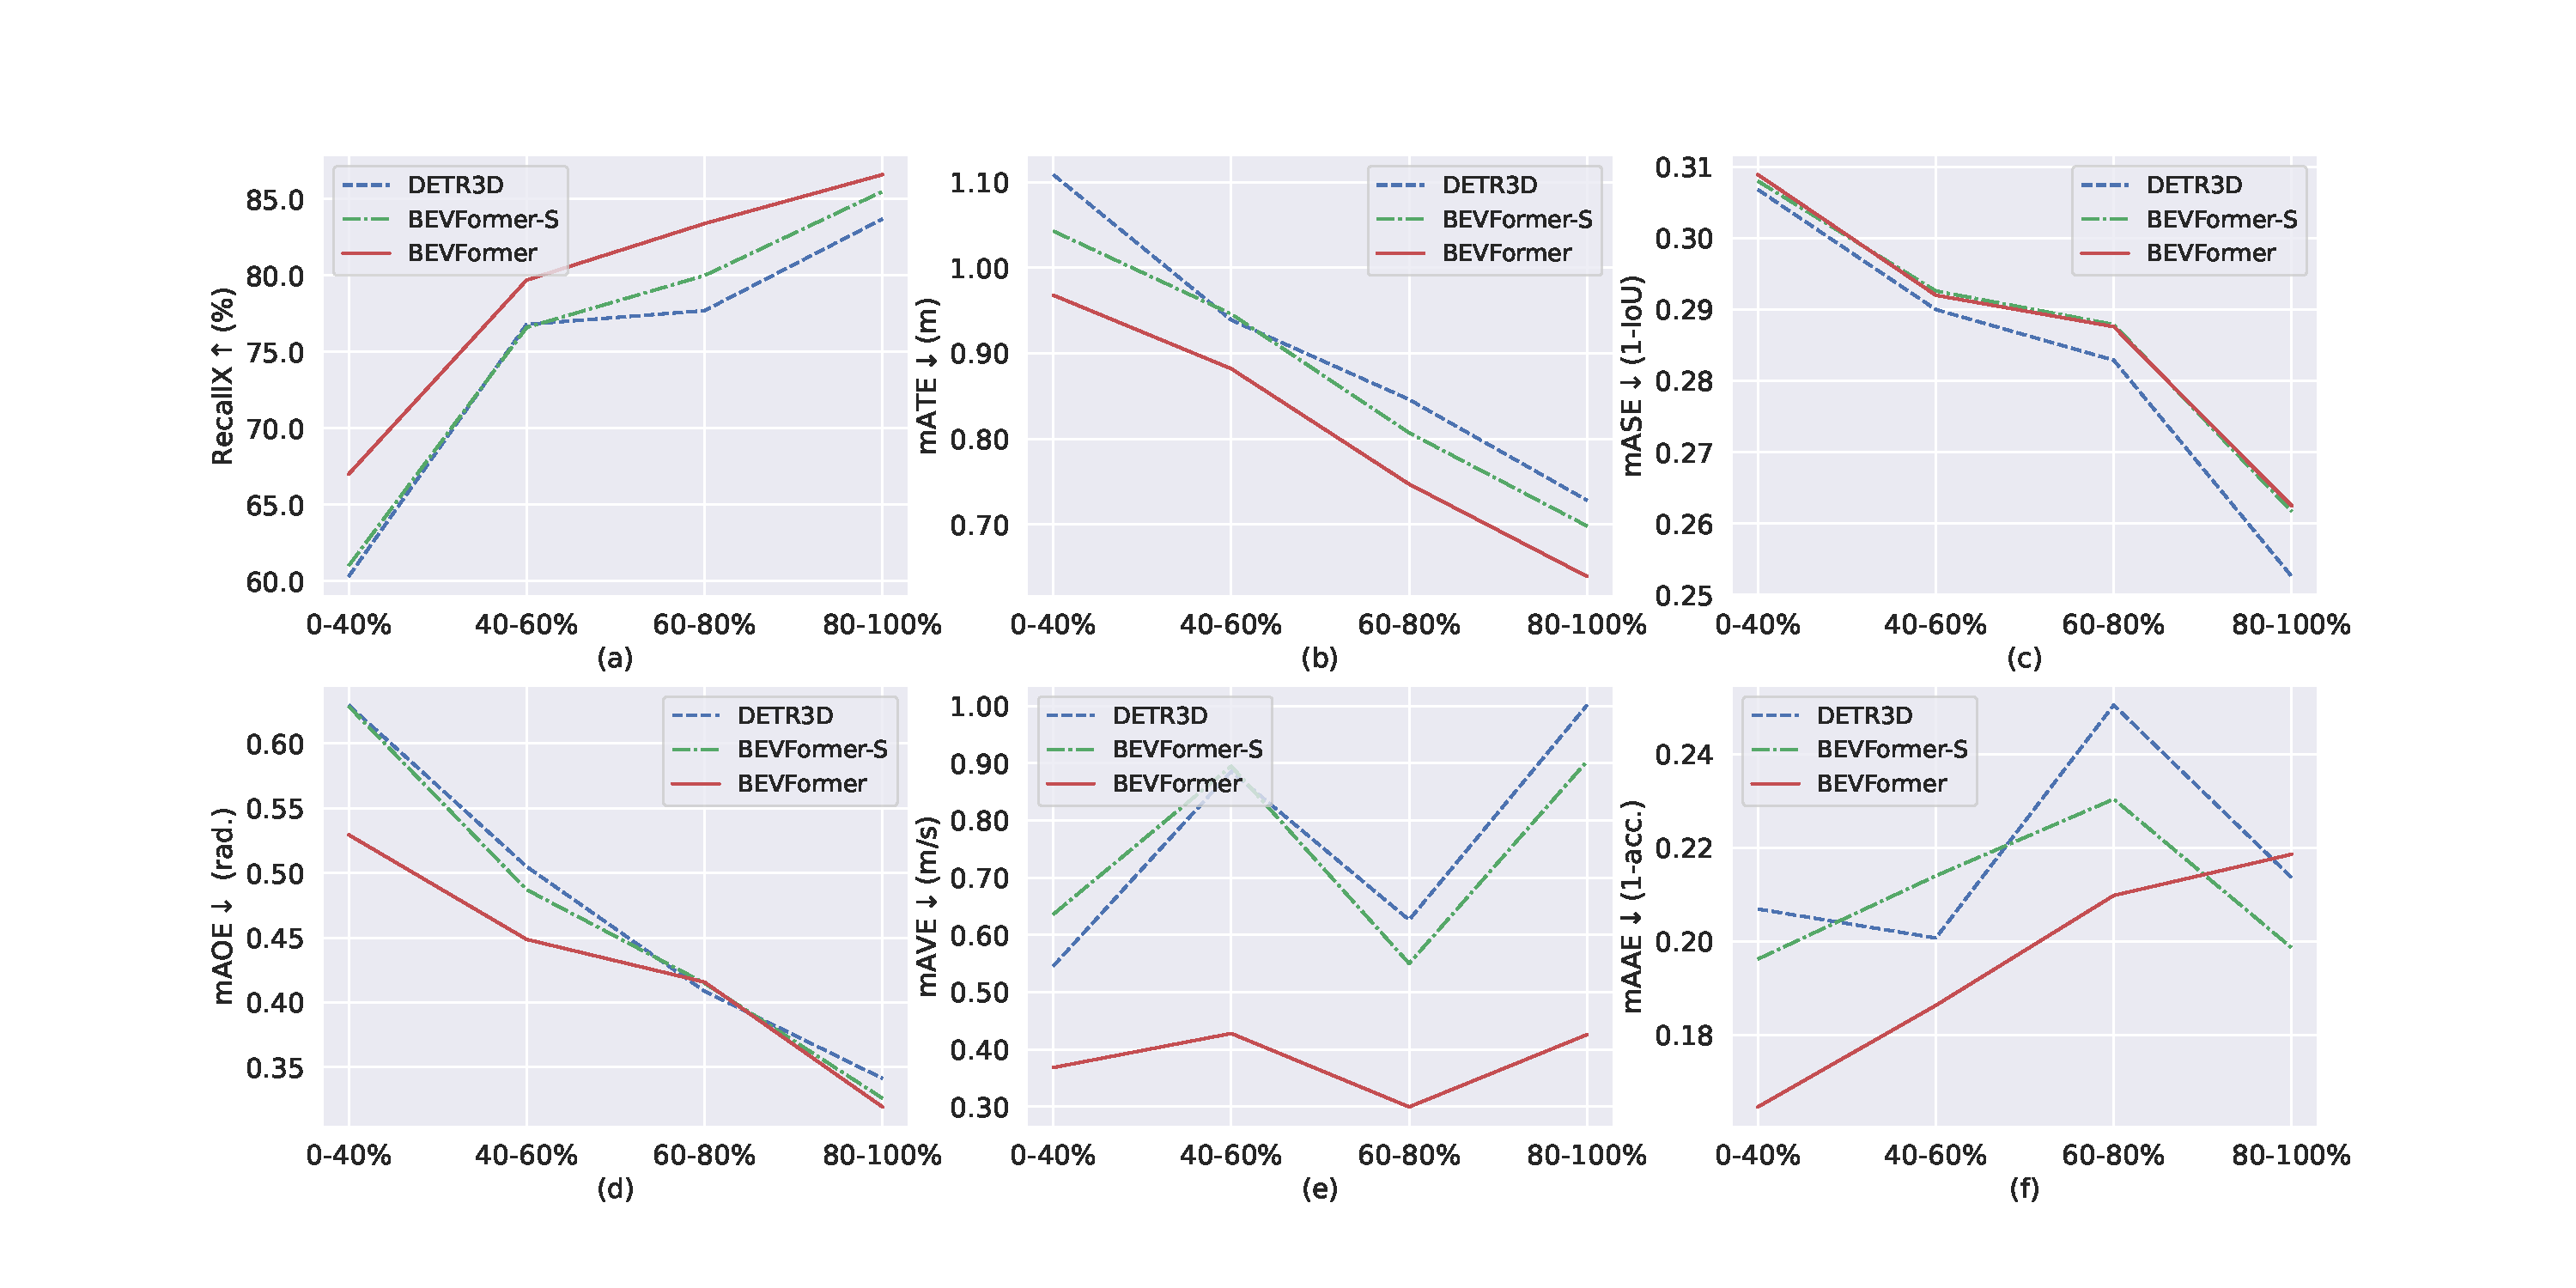
\includegraphics[width=\linewidth]{img/plt.pdf}
%\vspace{-5mm}
\caption{\textbf{不同可见度子集的检测结果。} 根据物体可见度将nuScenes \texttt{val}集划分为四个子集：\{0-40\%, 40-60\%, 60-80\%, 80-100\%\}的物体可见。 (a)：借助时序信息增强了BEVFormer在所有子集上的召回率，尤其在可见度最低的子集(0-40\%)上提升显著。 (b)、(d)和(e)：时序信息有助于提高平移、朝向和速度精度。 (c)和(f)：不同方法之间的尺度和属性误差差异较小。时序信息对物体尺度预测帮助有限。}
\label{fig:plt}

\end{figure}


\subsection{消融实验}


为深入探究不同模块的效果，在nuScenes \texttt{val}集上使用检测头进行消融实验。更多消融实验见附录。


\noindent\textbf{空间交叉注意力的有效性。}
为验证空间交叉注意力的效果，使用BEVFormer-S进行消融实验以排除时序信息的干扰，结果如表\ref{bevformer_s_abl}所示。
默认的空间交叉注意力基于可变形注意力。
为进行对比，还构建了另外两种使用不同注意力机制的基线：（1）使用全局注意力替换可变形注意力；（2）使每个查询仅与其参考点交互而非周围局部区域，这类似于先前的方法~\cite{Roddick2019OrthographicFT,rukhovich2022imvoxelnet}。
为进行更广泛的对比，还将BEVFormer替换为VPN~\cite{pan2020cross}和Lift-Splat~\cite{philion2020lift}提出的BEV生成方法。可以观察到，在可比的模型规模下，可变形注意力显著优于其他注意力机制。
全局注意力消耗过多GPU显存，而仅点交互的感知范围有限。
稀疏注意力通过与先验确定的感兴趣区域交互，平衡了感受野和GPU消耗，取得了更好的性能。


\noindent\textbf{时序自注意力的有效性。}
从表\ref{main_det}和表\ref{table:multi-tasks}可以观察到，在相同设置下BEVFormer以显著改进超越BEVFormer-S，尤其在具有挑战性的检测任务上。时序信息的效果主要体现在以下方面：（1）时序信息的引入极大提升了速度估计的精度；（2）使用时序信息后，物体位置和朝向的预测更加精确；（3）由于时序信息包含过去的物体线索，在严重遮挡的物体上获得了更高的召回率，如图\ref{fig:plt}所示。
为评估BEVFormer在不同遮挡程度物体上的性能，根据nuScenes提供的官方可见度标签将验证集划分为四个子集。在每个子集中，还计算了匹配时中心距离阈值为2米的所有类别的平均召回率。所有方法的最大预测框数量均为300，以公平比较召回率。
在仅有0-40\%物体可见的子集上，BEVFormer的平均召回率以超过6.0个百分点的优势超越BEVFormer-S和DETR3D。

\noindent\textbf{模型规模与延迟。}在表\ref{table:latency}中比较了不同配置的性能和延迟。从三个方面消融BEVFormer的规模，包括是否使用多尺度视图特征、BEV查询的形状和层数，以验证性能和推理延迟之间的权衡。可以观察到，配置C在BEVFormer中仅使用一个编码器层，达到了50.1\%的NDS，并将BEVFormer的延迟从原来的130ms降低到25ms。配置D采用单尺度视图特征、较小的BEV尺寸和仅有1个编码器层，推理时仅消耗7ms，尽管与默认配置相比损失了3.9个百分点。然而，由于多视角图像输入，限制效率的瓶颈在于骨干网络，适用于自动驾驶的高效骨干网络值得深入研究。
总体而言，架构可以适应多种模型规模，并灵活地权衡性能和效率。





\begin{table}[t] 
\begin{center}

\caption{
\textbf{不同模型配置在nuScenes \texttt{val}集上的延迟和性能。} 延迟在V100 GPU上测量，骨干网络为R101-DCN。输入图像尺寸为$900\!\times\!1600$。``MS''表示多尺度视图特征。
}
\setlength{\tabcolsep}{1.4mm}
\begin{tabular}{c| c c c | c c  c|c | c c}
\toprule
% \multirow{2}{*}{Clean} &\multirow{2}{*}{Mean} &
\multirow{2}{*}{方法}&
%\multirow{2}{*}{MS}&  \multirow{2}{*}{BEV Size} & \multirow{2}{*}{\#Layers}
\multicolumn{3}{c|}{BEVFormer规模}
 &  \multicolumn{3}{c|}{延迟 (ms)}&  \multirow{2}{*}{FPS} &\multirow{2}{*}{NDS$\uparrow$} &\multirow{2}{*}{mAP$\uparrow$}\\
&多尺度&BEV尺寸&层数& 骨干网络 & BEVFormer & 检测头&\\
%\multirow{2}{*}{Det} & \multirow{2}{*}{Seg}
%Method & Modality & NDS& mAP &  IOU$_{\rm Car}$
\midrule
BEVFormer & \cmark&$200\!\times\!200$ & 6 &391 & 130& 19 &1.7&\textbf{0.517}&\textbf{0.416}\\
\midrule
A & \xmark&$200\!\times\!200$ & 6 & 387& 87& 19&1.9&0.511&0.406\\
B & \cmark&$100\!\times\!100$ & 6 & 391& 53& 18&2.0&0.504&0.402\\
C & \cmark&$200\!\times\!200$ & 1 & 391& 25& 19&2.1&0.501&0.396\\
D & \xmark&$100\!\times\!100$ & 1 & 387& \textbf{7}& 18&\textbf{2.3}&0.478&0.374\\
\bottomrule

\end{tabular}

\label{table:latency}
\end{center}
\end{table}


\subsection{可视化结果}


在图\ref{fig:vis}中展示了一个复杂场景的检测结果。BEVFormer产生了令人印象深刻的结果，仅在少数小物体和远处物体上存在错误。更多定性结果见附录。


\begin{figure}[t]
\centering
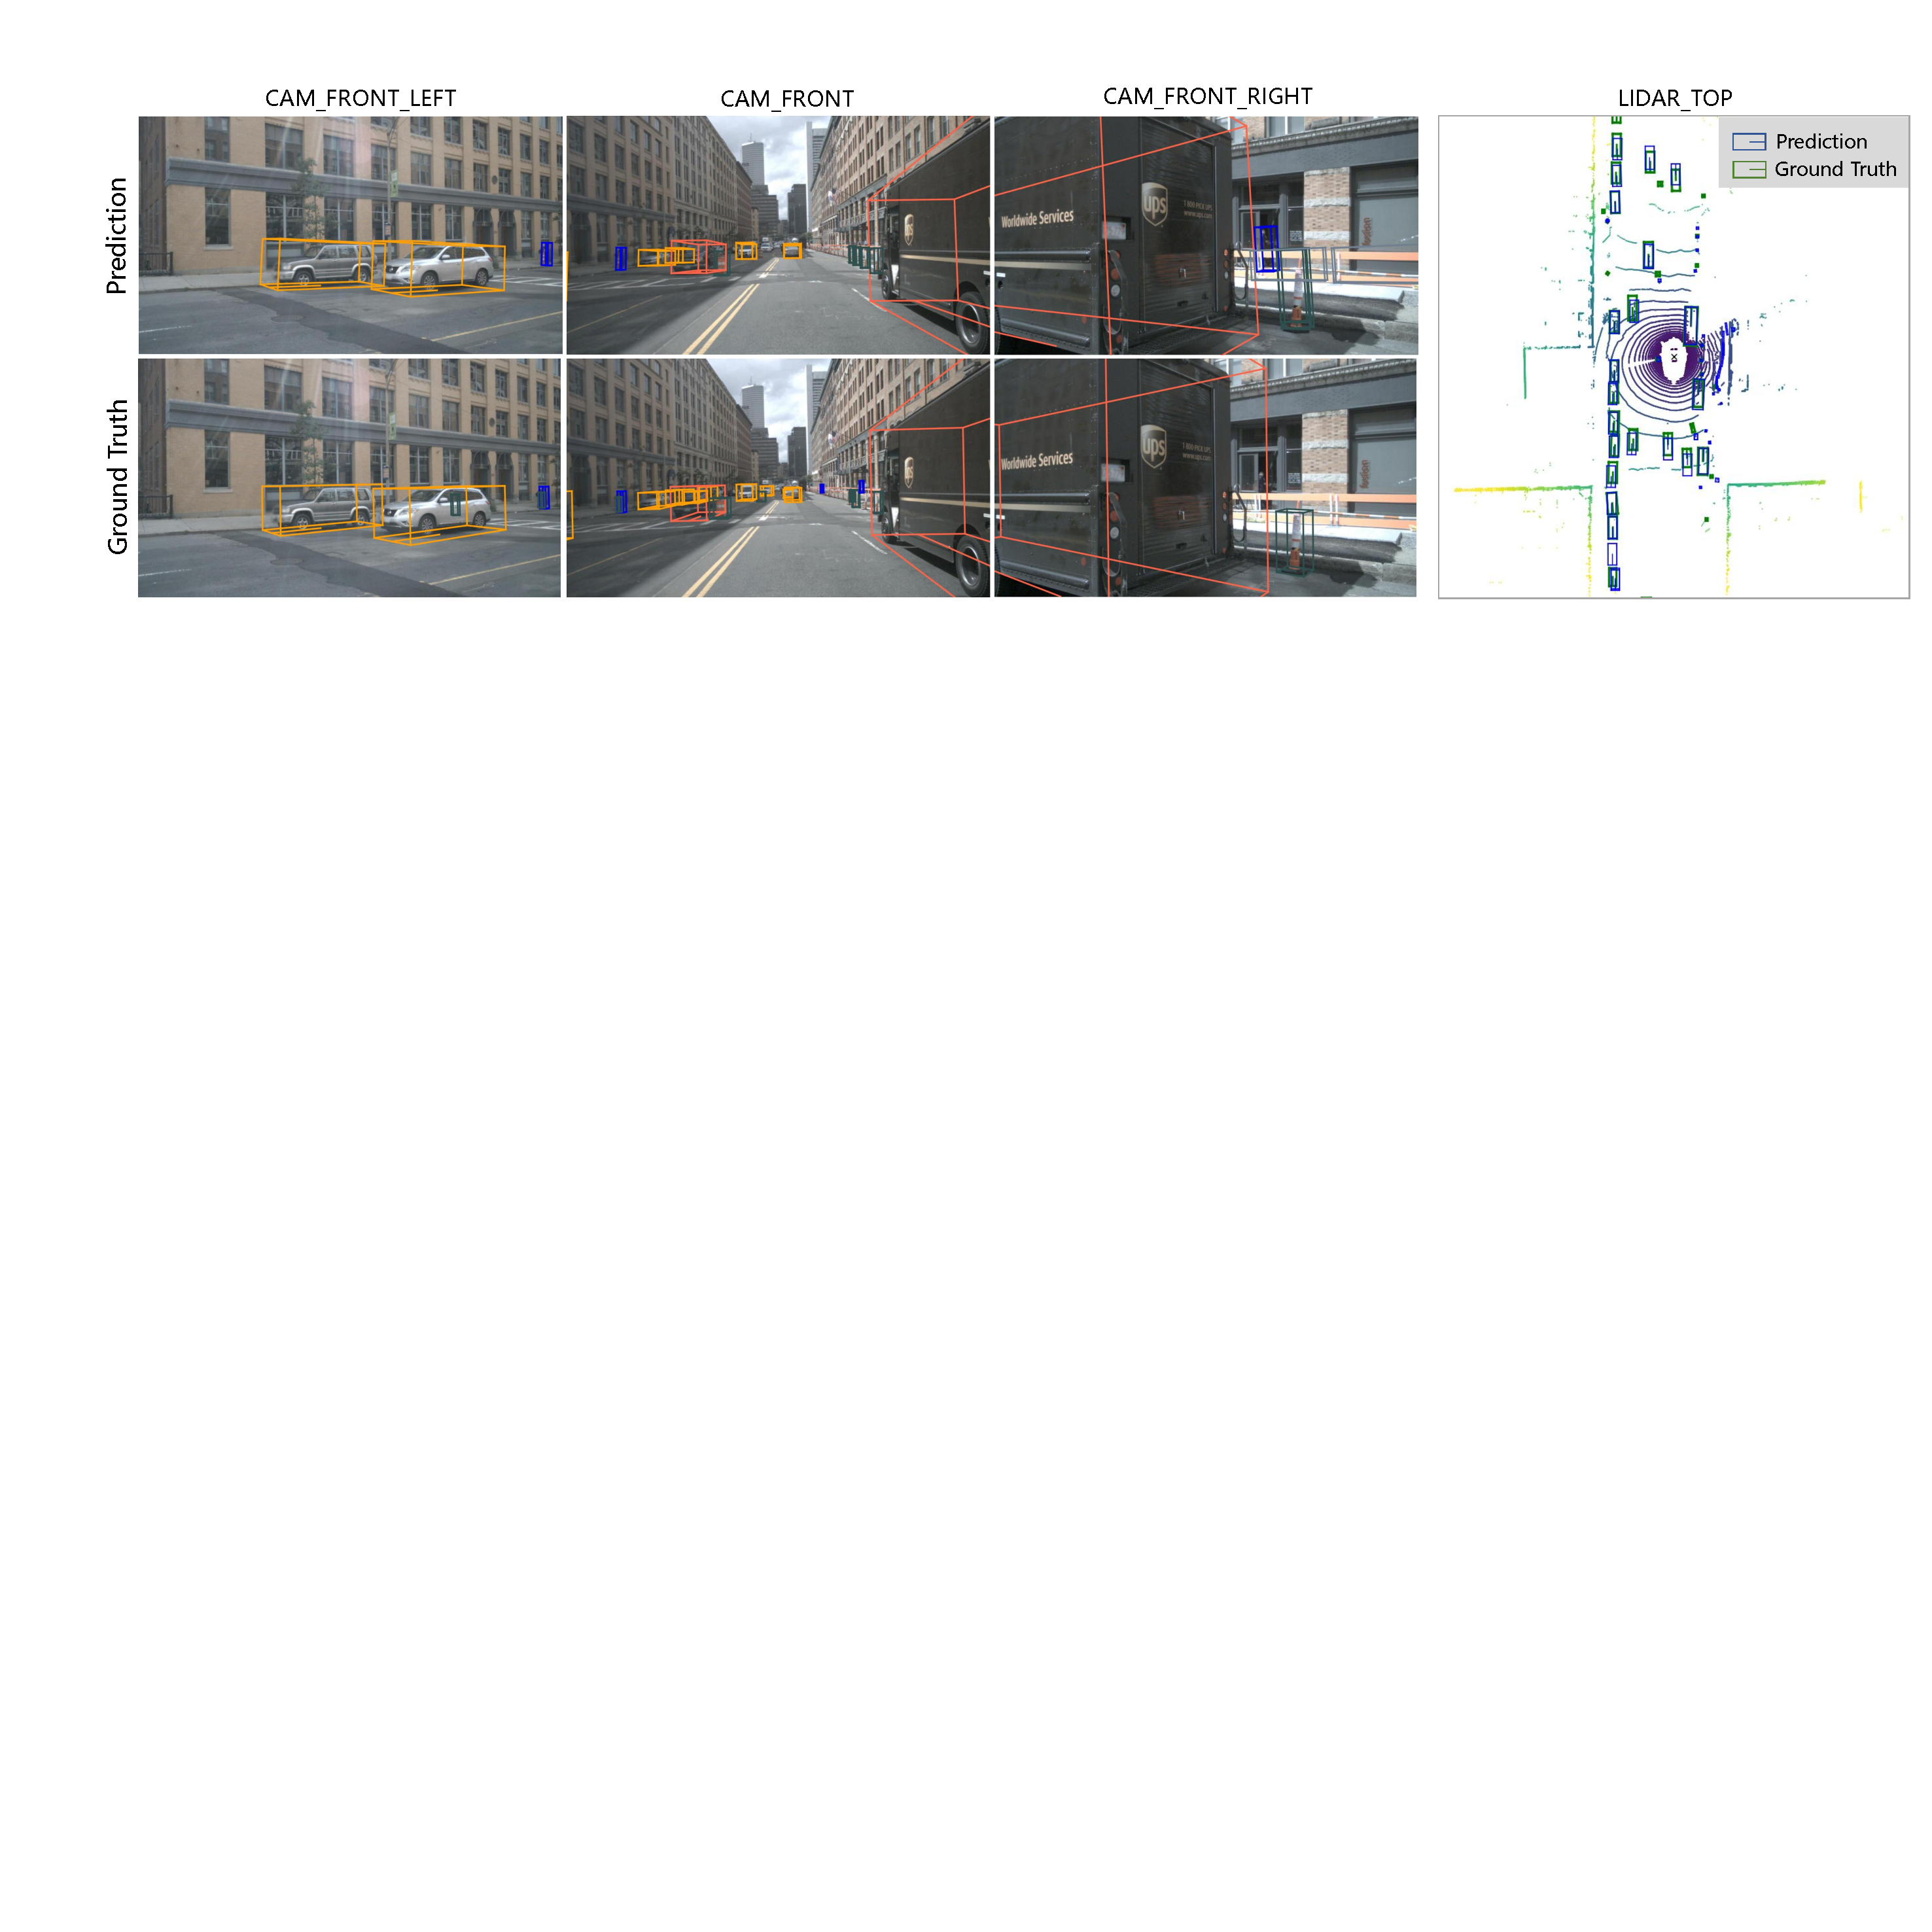
\includegraphics[width=\linewidth]{img/visual2.pdf}
\caption{\textbf{BEVFormer在nuScenes \texttt{val}集上的可视化结果。} 展示了多相机图像和鸟瞰视图中的3D边界框预测结果。
}
\label{fig:vis}

\end{figure}



\section{讨论与结论}

本文提出了BEVFormer，用于从多相机输入生成鸟瞰视图特征。BEVFormer能够高效聚合空间和时序信息，生成强大的BEV特征，同时支持3D目标检测和地图分割任务。

\noindent\textbf{局限性。}目前，基于相机的方法在效果和效率上与基于LiDAR的方法仍存在一定差距。从2D信息精确推理3D位置仍然是基于相机的方法长期面临的挑战。

\noindent\textbf{更广泛的影响。}
BEVFormer证明了利用多相机输入的时空信息可以显著提升视觉感知模型的性能。BEVFormer展示的优势，如更精确的速度估计和更高的低可见度物体召回率，对于构建更好、更安全的自动驾驶系统及其相关应用至关重要。相信BEVFormer只是后续更强大的视觉感知方法的一个基线，基于视觉的感知系统仍有巨大潜力有待挖掘。 


\bibliographystyle{splncs04}
\bibliography{egbib}

\clearpage

\section*{附录}
\appendix


\section{实现细节}
本节提供所提方法和实验的更多实现细节。

\subsection{训练策略}





参照先前方法~\cite{wang2022detr3d,zhu2020deformable}，
所有模型训练24个轮次，每个GPU的批大小为1（包含6张视图图像），学习率为$2\!\times\!10^{-4}$，骨干网络的学习率乘数为0.1，使用余弦退火~\cite{Loshchilov2017SGDRSG}衰减学习率。采用AdamW~\cite{Loshchilov2019DecoupledWD}优化模型，权重衰减为$1\!\times\!10^{-2}$。

\subsection{VPN与Lift-Splat}
本文使用VPN~\cite{pan2020cross}和Lift-Splat~\cite{philion2020lift}作为两个基线方法。为公平比较，骨干网络和任务头与BEVFormer相同。

\noindent\textbf{VPN.}使用官方代码\footnote{https://github.com/pbw-Berwin/View-Parsing-Network}。受限于MLP的巨大参数量，VPN难以生成高分辨率BEV（如200$\times$200）。
为与VPN进行比较，本文通过两个视图转换层将单尺度视图特征转换为低分辨率（$50\!\times\!50$）的BEV。

\noindent\textbf{Lift-Splat.}为与BEVFormer在可比参数量下进行公平比较，对Lift-Splat\footnote{https://github.com/nv-tlabs/lift-splat-shoot}的相机编码器增加了两个额外的卷积层。其他设置保持不变。



\subsection{任务头} 

%\begin{figure}

%\end{figure}

\begin{wrapfigure}{r}{0.35\linewidth}
    \vspace{-35pt}
    %\centering
    \renewcommand{\captionlabelfont}{\scriptsize}
    \begin{center}
    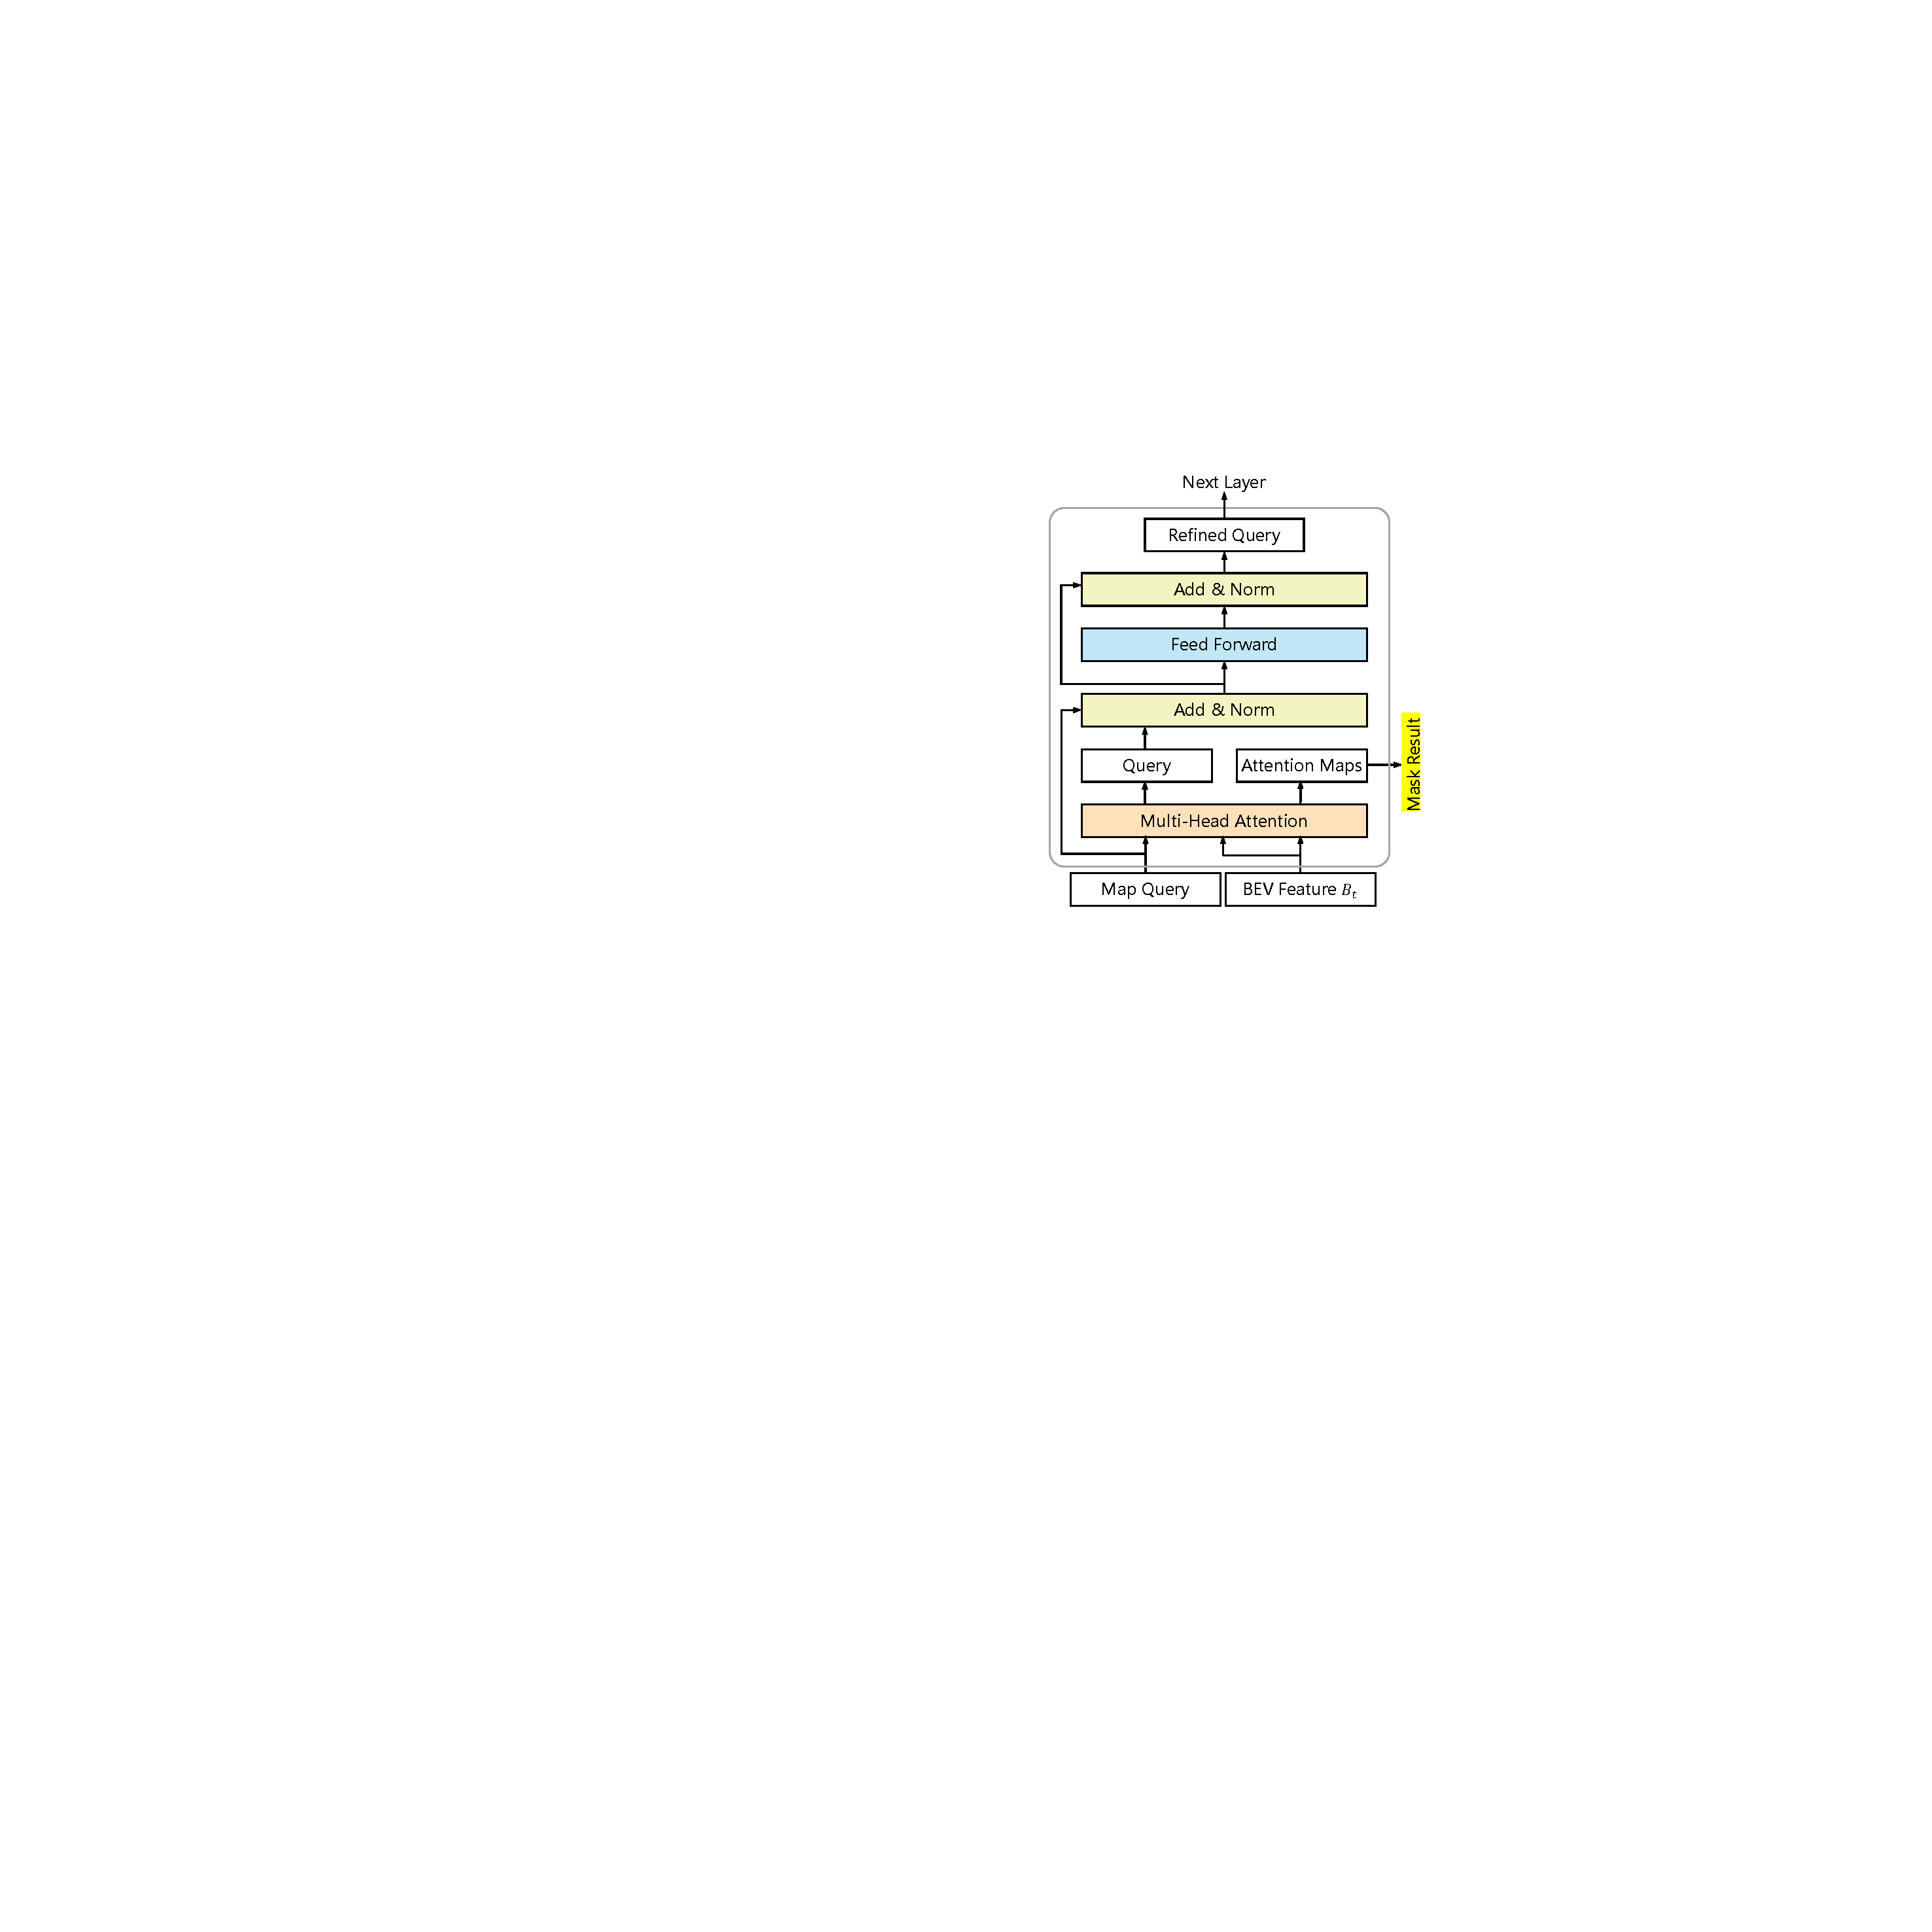
\includegraphics[width=\linewidth]{img/mask_decoder_arch.pdf}
    \caption{\scriptsize \textbf{
    % Model Architecture.
    BEVFormer的分割头（掩码解码器）。
    }}
    \label{fig:appdendix_arch}
    \end{center}
    \vspace{-40pt}
\end{wrapfigure}
\textbf{检测头。}为每个3D边界框预测10个参数，
包括框尺度的3个参数$(l,w,h)$，中心位置的3个参数$(x_o,y_o,z_o)$，物体偏航角$\theta$的2个参数（cos($\theta$), sin($\theta$)），以及速度的2个参数$(v_x,v_y)$。训练阶段仅使用$L_1$损失和$L_1$代价。参照~\cite{wang2022detr3d}，使用900个目标查询，推理时保留置信度最高的300个预测框。

\noindent\textbf{分割头。}
如图\ref{fig:appdendix_arch}所示，对于语义图的每个类别，借鉴\cite{li2021panoptic}中的掩码解码器，使用一个可学习查询表示该类别，基于标准多头注意力的注意力图生成最终分割掩码。

\subsection{空间交叉注意力}

\noindent\textbf{全局注意力。}除了可变形注意力~\cite{zhu2020deformable}，空间交叉注意力也可以通过全局注意力（即标准多头注意力）~\cite{vaswani2017attention}实现。使用全局注意力最直接的方式是让每个BEV查询与所有多相机特征交互，这种概念实现不需要相机标定。
然而，这种直接方式的计算成本不可承受。因此，仍然利用相机内参和外参来决定每个BEV查询应当交互的命中视图。该策略使得一个BEV查询通常仅与一个或两个视图交互而非全部视图，从而使在空间交叉注意力中使用全局注意力成为可能。值得注意的是，与其他依赖精确相机内参和外参的注意力机制相比，全局注意力对相机标定更加鲁棒。


\section{相机外参鲁棒性}
BEVFormer依赖相机内参和外参获取2D视图上的参考点。在自动驾驶系统部署阶段，由于标定误差、相机偏移等各种原因，外参可能存在偏差。如图\ref{fig:noise}所示，展示了模型在不同相机外参噪声水平下的结果。
与BEVFormer-S (point)相比，BEVFormer-S使用基于可变形注意力~\cite{zhu2020deformable}的空间交叉注意力，在参考点周围采样特征，而非仅与参考点交互。
%
借助可变形注意力，BEVFormer-S的鲁棒性强于BEVFormer-S (point)。例如，在噪声水平为4时，BEVFormer-S的NDS下降了15.2\%（计算方式为$1-\frac{0.380}{0.448}$），而BEVFormer-S (point)的NDS下降了17.3\%。与BEVFormer-S相比，BEVFormer仅下降14.3\%的NDS，表明时序信息也能提升对相机外参的鲁棒性。
参照~\cite{philion2020lift}，结果表明当使用含噪声的外参训练BEVFormer时，BEVFormer (noise)具有更强的鲁棒性（仅下降8.9\% NDS）。使用基于全局注意力的空间交叉注意力时，即使在相机外参噪声水平4下，BEVFormer (global)也具备很强的抗干扰能力（NDS下降4.0\%）。原因在于不需要利用相机外参为BEV查询选择感兴趣区域。

值得注意的是，在最严苛的噪声条件下，BEVFormer-S (global)甚至优于BEVFormer-S（38.8\% NDS \emph{vs.} 38.0\% NDS）。

\begin{figure}[t]
\centering

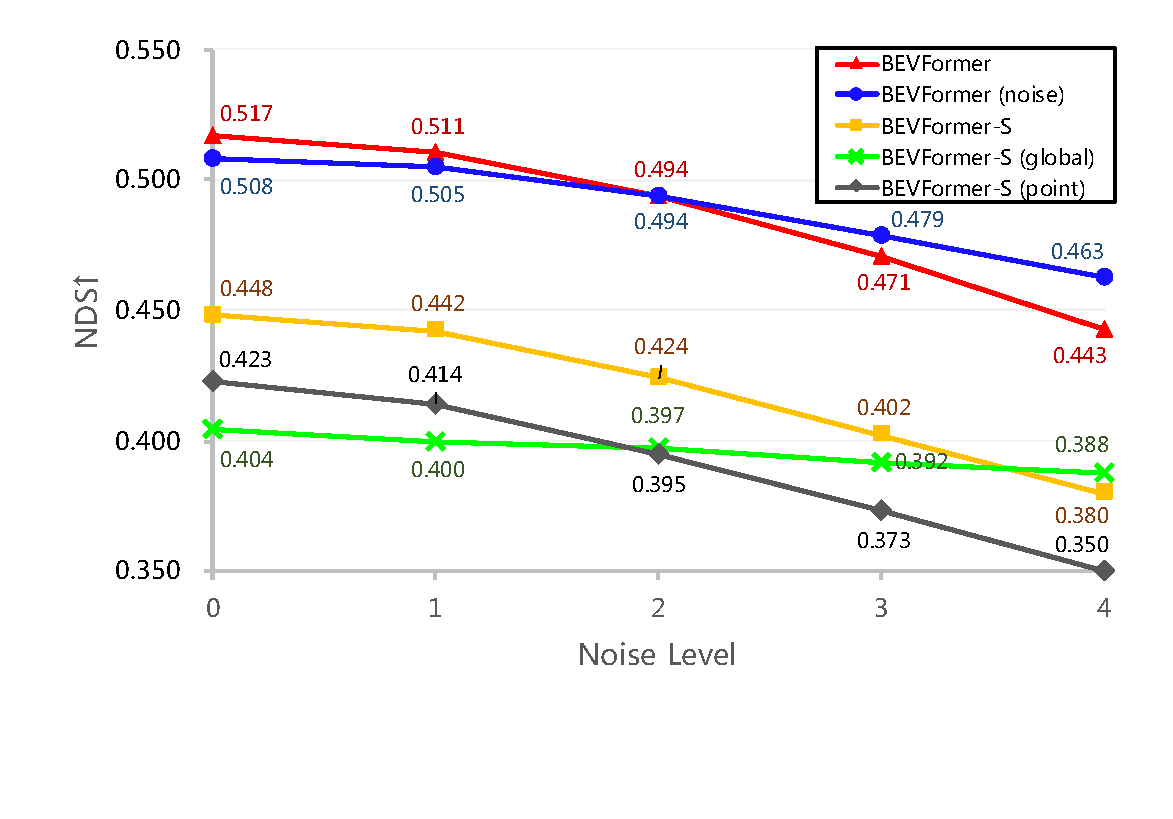
\includegraphics[width=0.75\linewidth]{img/robust.pdf}
\caption{\textbf{不同相机外参噪声水平下各方法在nuScenes val集上的NDS。} 对于第$i$级噪声，旋转噪声从均值为0、方差为$i$的正态分布中采样（旋转噪声单位为度，各轴噪声独立），平移噪声从均值为0、方差为$5i$的正态分布中采样（平移噪声单位为厘米，各方向噪声独立）。
``BEVFormer''是默认版本。
``BEVFormer (noise)''使用含噪声外参（噪声水平=1）训练。
``BEVFormer-S''是BEVFormer的静态版本，空间交叉注意力由可变形注意力~\cite{zhu2020deformable}实现。``BEVFormer-S (global)''是BEVFormer-S的空间交叉注意力由全局注意力（即标准多头注意力）~\cite{vaswani2017attention}实现。``BEVFormer-S (point)''是BEVFormer-S使用点空间交叉注意力，通过移除预测的偏移量和权重将可变形注意力的交互目标从局部区域退化为仅参考点。}
\label{fig:noise}

\end{figure}



\iffalse
\section{零样本迁移}

使用nuScenes~\cite{caesar2020nuscenes}数据训练BEVFormer，但在Waymo开放数据集上评估3D目标检测任务。由于不同域、不同感知范围和不同相机（包括不同的内参和外参、不同数量的相机、不同的水平视场角），这极具挑战性。
使用nuScenes指标，BEVFormer在车辆类别上达到7.6\%的NDS，远低于在Waymo开放数据集上训练得到的42.6\% NDS。如图\ref{fig:waymo_zero_shot}所示，BEVFormer在某些场景中可以检测出不错的结果。然而，总体而言它产生了过多的假阳性结果，且召回率很低。这一具有挑战性的任务仍需在未来的工作中进一步探索。
\begin{figure}[h]
\centering
\includegraphics[width=0.8\linewidth]{img/waymo_zero_shot.pdf}
\caption{在Waymo开放数据集上的可视化结果。黄色和蓝色边界框分别为真实值和预测结果，置信度阈值设为0.1。
仅使用nuScenes训练数据训练BEVFormer。BEVFormer能够检测出一些合理的边界框。}
\label{fig:waymo_zero_shot}

\end{figure}
\fi

\section{消融实验}

\noindent\textbf{训练中帧数量的影响。} 表\ref{tab:table1_a}展示了训练中帧数量的影响。可以看到，nuScenes val集上的NDS随帧数增加持续上升，并在帧数$\ge 4$时趋于平稳。因此，实验默认将训练帧数设为4。



\noindent\textbf{部分设计的影响。} 表\ref{tab:table1_b}展示了多项消融实验的结果。比较\#1和\#4，将历史BEV特征与自车运动对齐对于表示与当前BEV查询相同的几何场景至关重要（51.0\% NDS \emph{vs.} 51.7\% NDS）。比较\#2和\#4，从5帧中随机采样4帧是一种有效的数据增强策略，可提升性能（51.3\% NDS \emph{vs.} 51.7\% NDS）。与仅使用BEV查询预测时序自注意力模块中的偏移量和权重（见\#3）相比，同时使用BEV查询和历史BEV特征（见\#4）包含更多关于过去BEV特征的线索，有利于位置预测（51.3\% NDS \emph{vs.} 51.7\% NDS）。


\begin{table}

\begin{minipage}[!t]{0.5\linewidth}

\centering
\captionsetup{width=.95\textwidth}
\caption{\textbf{不同训练帧数下模型在nuScenes val集上的NDS。} ``\#Frame''表示训练帧数。
}
\begin{center}

\setlength{\tabcolsep}{2.0mm}
\begin{tabular}[t]{c| c c c}
\toprule

\#Frame & NDS$\uparrow$ & mAP$\uparrow$ &mAVE$\downarrow$\\
\midrule
1 & 0.448 & 0.375 &0.802\\ 
2 & 0.490 &0.388 & 0.467\\
3 & 0.510 & 0.410 &0.423 \\
4 & \textbf{0.517} & \textbf{0.416} & 0.394\\
5 & \textbf{0.517} & 0.412 & \textbf{0.387}\\
\bottomrule
\end{tabular}
\label{tab:table1_a}
\end{center}
\end{minipage}%
\begin{minipage}[!t]{0.5\linewidth}
\centering
\captionsetup{width=.95\textwidth}
\caption{\textbf{nuScenes val集上的消融实验。} ``A.''表示将历史BEV特征与自车运动对齐。``R.''表示从5个连续帧中随机采样4帧。``B.''表示同时使用BEV查询和历史BEV特征预测偏移量和权重。}
\renewcommand{\arraystretch}{0.88}
\setlength{\tabcolsep}{0.5mm}
\begin{center}
\addtolength{\tabcolsep}{4pt}
\begin{tabular}[t]{c | c c c |c c}
\toprule

\#   & A. & R. & B. & NDS$\uparrow$ & mAP$\uparrow$ \\
\midrule
%1 &  \xmark & \cmark & \cmark & \cmark & 0.512 & 0.412\\
1 & \xmark & \cmark & \cmark & 0.510& 0.410\\
2  & \cmark & \xmark & \cmark &0.513 & 0.410\\
3  & \cmark & \cmark & \xmark &  0.513 & 0.404\\
\midrule
4 &\cmark & \cmark & \cmark &  \textbf{0.517} & \textbf{0.416}\\
\bottomrule
\end{tabular}


\label{tab:table1_b}
\end{center}
\end{minipage}



\label{tab:table1}

\end{table}

\section{可视化}

如图\ref{fig:static_vs_video}所示，比较了BEVFormer与BEVFormer-S。借助时序信息，BEVFormer成功检测到两辆被遮挡的公交车。还在图\ref{fig:visual_4000}中展示了目标检测和地图分割结果，可以看到检测结果和分割结果高度一致。在图\ref{fig:mask}中提供了更多地图分割结果，可以看出借助BEVFormer生成的强大BEV特征，通过简单的掩码解码器即可很好地预测语义图。
\vspace{16mm}
\begin{figure}[h]
\centering
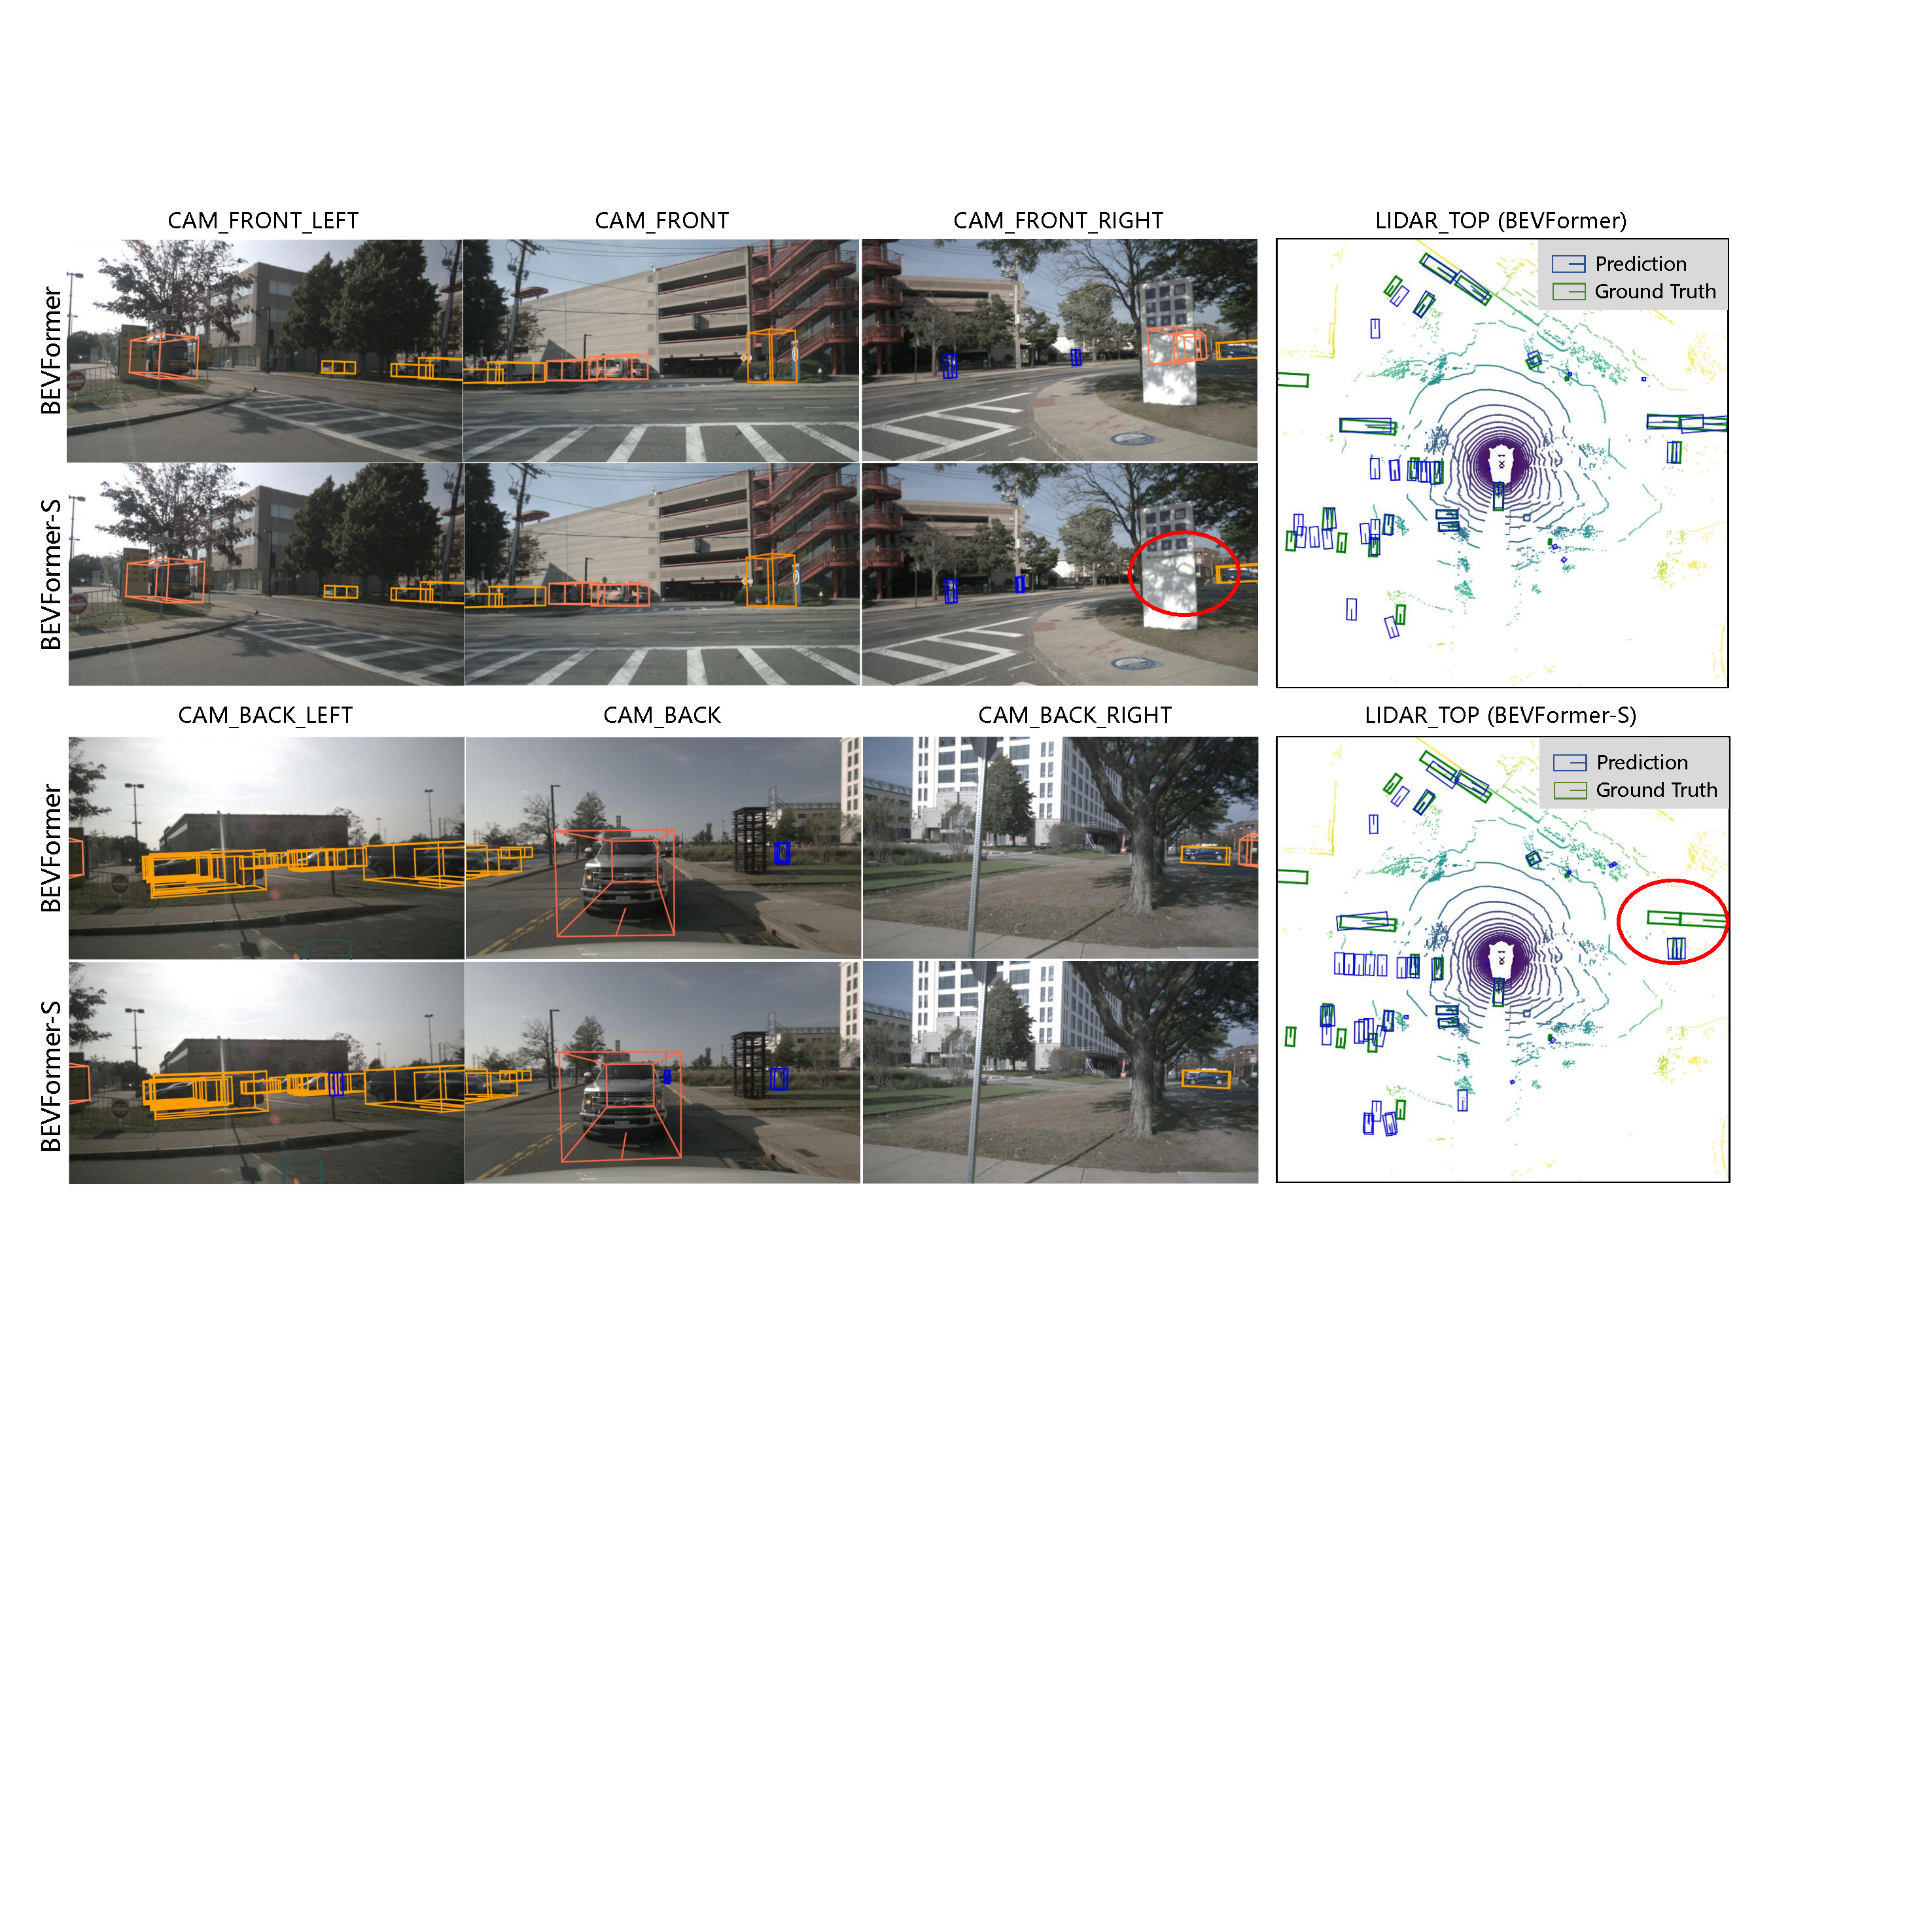
\includegraphics[width=\linewidth]{img/static_vs_video.pdf}
\caption{\textbf{BEVFormer与BEVFormer-S在nuScenes val集上的对比。} 可以观察到BEVFormer能够检测到严重遮挡的物体，而这些物体在BEVFormer-S的预测结果中被遗漏（红色圆圈标注）。
}
\label{fig:static_vs_video}
\end{figure}


\begin{figure}[b]
\centering
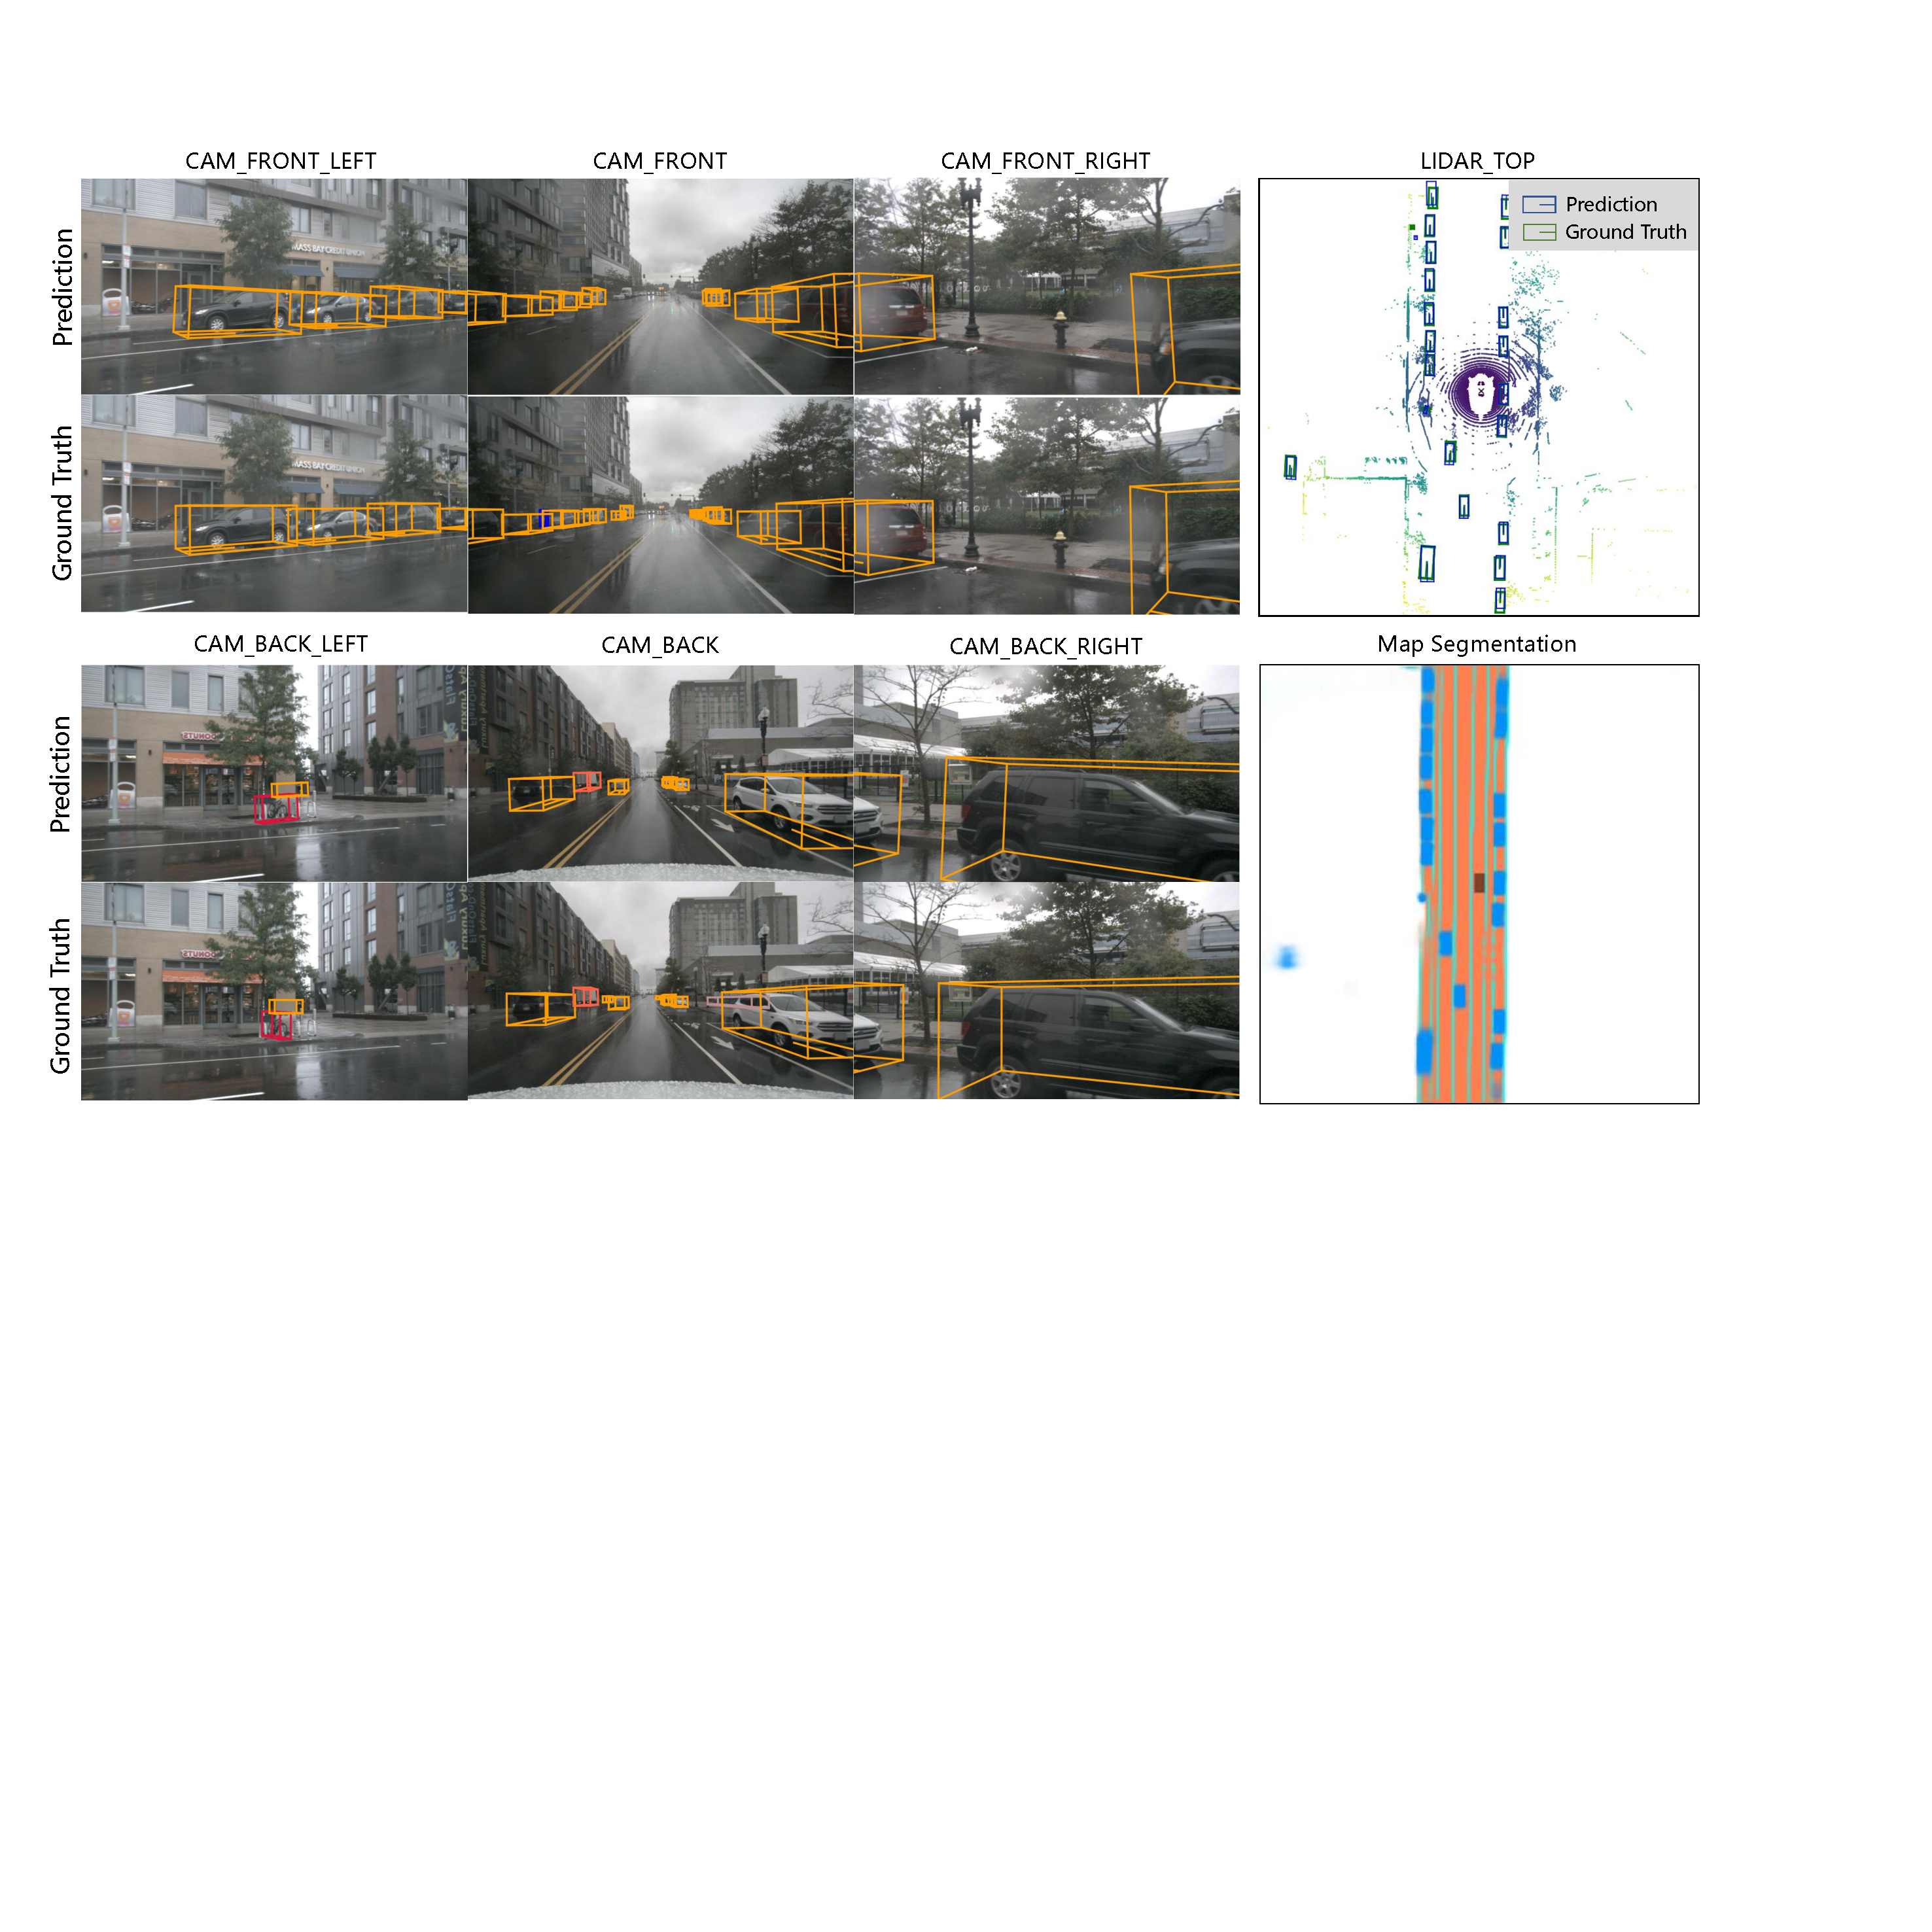
\includegraphics[width=\linewidth]{img/visual_4000.pdf}
\caption{\textbf{目标检测和地图分割任务的可视化结果。} 车辆、道路和车道分割分别用蓝色、橙色和绿色表示。
}
\label{fig:visual_4000}
\end{figure}


\begin{figure}[h]
\centering
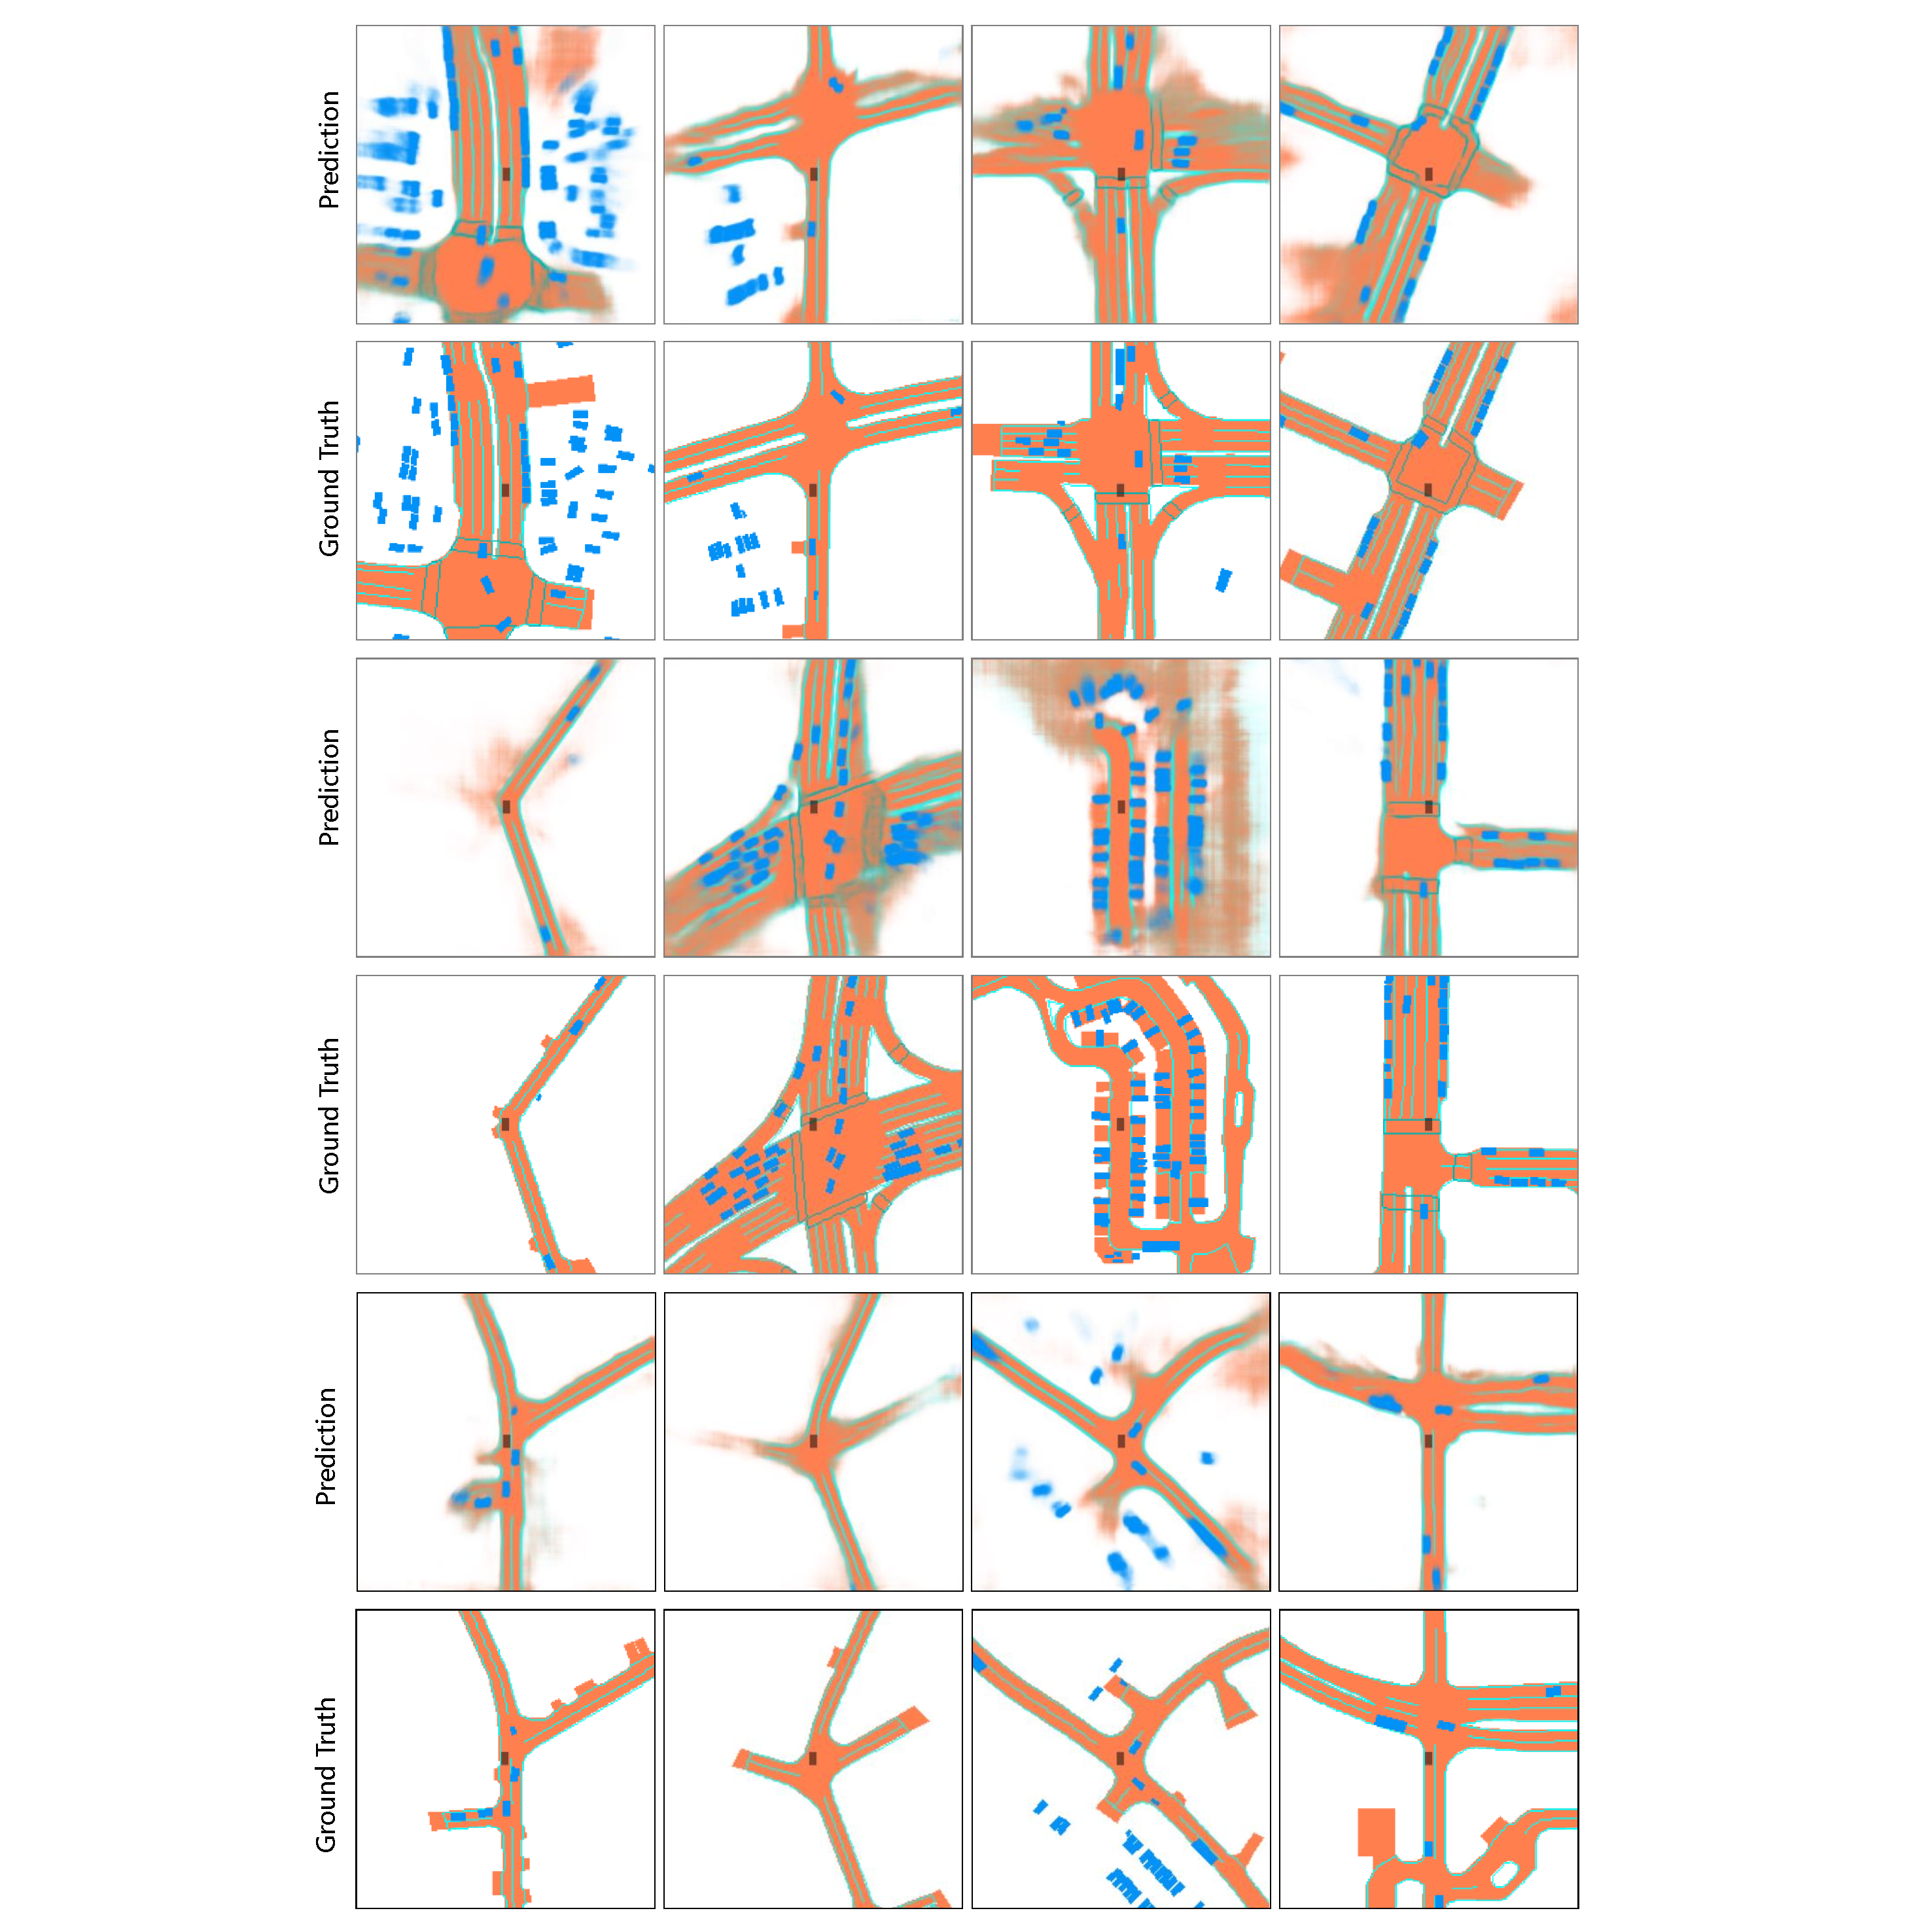
\includegraphics[width=\linewidth]{img/seg_mask.pdf}
\caption{\textbf{地图分割任务的可视化结果。} 车辆、道路、人行横道和车道分割分别用蓝色、橙色、青色和绿色表示。
}
\label{fig:mask}
\end{figure}



\end{document}
